\documentclass[a4paper, 12pt, openright, oneside, german, french, brazil, english]{abntex2}
\usepackage[brazil]{babel}
\usepackage{graphicx}
\usepackage[utf8]{inputenc}
\usepackage{graphicx}
\usepackage{wrapfig}
\usepackage{lscape}
\usepackage{rotating}
\usepackage{epstopdf}
\usepackage[alf,abnt-and-type=&]{abntex2cite}
\usepackage[a4paper, left=2cm, right=2cm, top=2cm, bottom=2cm]{geometry}
\usepackage{indentfirst}
\usepackage{longtable}
\pagestyle{plain}

\titulo{The social construction of quality in a Brazilian Classical Music market}
\autor{Neylson J. B. F. Crepalde}
\data{January, 2018}
\instituicao{UNIVERSIDADE FEDERAL DE MINAS GERAIS
	\par
	Faculdade de Filososia e Ciências Humanas}
\local{Belo Horizonte}
\orientador{Dr. Silvio Salej Higgins (PPGS -- UFMG)}

\coorientador{Dr. Emmanuel Lazega (CSO, SciencesPo -- Paris)}
% \preambulo{Projeto de Pesquisa apresentado ao Programa de Pós-Graduação em Sociologia da UFMG como requisito para ingresso no Programa Doutorado Sanduíche no Exterior (PDSE).}
%\tipotrabalho{Tese (doutorado)}


\begin{document}
\pretextual
\imprimirfolhaderosto

 \listoffigures
 \listoftables
\newpage
\tableofcontents


	
	\textual
	\chapter{Introduction}

	%Para que o produto final por excelência de uma orquestra, a saber o concerto, venha a existir e chegue ao seu destino, o público, uma série de atores se envolvem em diversos processos de cooperação e mobilizam uma série de recursos construindo um sistema de produção em rede, ou o que Howard Becker chamaria de um ``mundo da arte'' (\textit{Art World}). Para \citeonline[p. 1, tradução do autor]{becker2008art}, ``a existência de mundos da arte, bem como o modo como sua existência afeta tanto a produção quanto o consumo de obras de arte, sugere uma abordagem sociológica para as artes'' \footnote{The existence of art worlds, as well as the way their existence affects both the production and consumption of art works, suggests a sociological approach to the arts.}.

	In order for the final product of an orchestra, the concert, to come into existence and reach its destination, the public, a number of actors engage in multiple cooperation processes and mobilize multiple resources building a production network system, or what Howard Becker would call an ``Art World''. To \citeonline[p. 1]{becker2008art}, ``the existence of art worlds, as well as the way their existence affects both the production and consumption of art works, suggests a sociological approach to the arts''.
	
	%Por outro lado, se prestamos atenção à dinâmica comum aos mercados, o que percebemos com maior facilidade é um ambiente altamente concorrencial. O fenômeno supracitado é abordado por \citeonline{lazega2009theorie} de uma perspectiva distinta: no mundo concorrencial, os atores se veem constantemente em situações em que buscam a estabilidade do mercado tornando-o viável. Isso não acontece simplesmente de acordo com a lei da oferta e da demanda mas a partir do posicionamento dos produtores numa escala de qualidade que diferencia seus produtos. Para que isso seja possível, a concorrência total é inviável já que existe uma parcela de interdependência entre produtores. Essa visão está ancorada na perspectiva relacional a qual concebe mercados como estruturas sociais, empresas, Estados, etc., como estruturas em rede \cite{white2008,white2002markets,lazega2014redes}.

	On the other hand, if we pay attention to the common market dynamics, what we can easily perceive is a highly competitive environment. The mentioned phenomenon is approached by \citeonline{lazega2009theorie} from a different perspective: in the competitive world, actors constantly see themselves in situations where they seek market's stability. This does not happen simply because of the law of supply and demand but from producers positioning in a quality scale that differentiates their products. For this to be possible, full competition is not viable since there is some interdependence between producers. This vision is anchored on the relational perspective which conceives markets as social structures and enterprises, states, etc. as network structures \cite{white2008,white2002markets,lazega2014redes}.


	%O foco deste trabalho é descortinar o mercado da música de concerto. Esse mercado ainda permanece fora do interesse convencional de economistas, sociólogos e demais estudiosos dos mercados, talvez por uma mera obra do acaso, talvez por sua alta complexidade e especificidade. Antes de apresentar nossas perguntas de pesquisa e nossos objetivos, faz-se necessário uma imersão na literatura de base realizando uma revisão tão profunda quanto possível. Após essa revisão, tentaremos extrair da observação da própria literatura (considerando o que já está postulado e, sobretudo, as lacunas existentes) os rumos de nossa investigação.
	
	The main goal of this investigation is to uncover classical music market. This market still remains out of the common sense interest of economists, sociologists and other market scholars, maybe by chance, maybe by its high complexity and specificity. To guide this investigation, a theoretical framework is proposed aggregating four elements: two economic sociology theories, one regarding quality as the main discipline of production markets \cite{white2002markets}, other stating the centrality of the State \cite{fligstein2002architecture}, normative isomorphisms concept \cite{dimaggio1983iron} and the brand new theory of multilevel networks \cite{lazega2016multilevel}.
	
	Before presenting our research questions and our goals, it is necessary to do an immersion in the specific literature in order to make a theoretical review as deep as possible. Afterwards, we will try to extract from the observation of the literature (considering what is already postulate and, above all, the identified gaps) the direction of our investigation.

	%Desse modo, iniciaremos o trabalho apresentado brevemente uma pesquisa bibliográfica realizada em duas das principais bases de produção acadêmica disponíveis na área de sociologia e economia. Encontramos que a produção científica sobre o mercado da música de concerto nos últimos 30 anos é ínfima. Depois, investigaremos na teoria econômica o conhecimento já sedimentado sobre bens culturais buscando entender os desafios colocados por nosso objeto de pesquisa. No terceiro capítulo, apresentaremos o framework teórico adotado para as análises, qual seja, a Análise de Redes Sociais (\textit{Social Network Analysis})\footnote{Muito embora, antecipamos, as ferramentas conhecidas como \textit{social network analysis} não constituem uma teoria geral do mundo que dedutivamente se aplique a qualquer realidade complexa. Trata-se, aqui, de um conjunto de ferramentas metodológicas aliadas a uma concepção de relações sociais.}. No quarto capítulo apresentaremos o desenho de pesquisa explicitando que tipo de dados intencionamos coletar, os procedimentos adotados, as formas de análises e os resultados esperados. Por fim, apresentamos uma investigação preliminar iniciada com uma das orquestras da cidade de Belo Horizonte bem como as considerações finais deste projeto.

	Therefore, we will begin our work presenting the results of our biliographic research. It was made in two of the main abstract bases in sociology and economics\footnote{Sociological Abstracts and Econlit.}.

	%Para o autor, ``a construção coletiva da qualidade implica que a viabilidade do mercado vem do coletivo, e que é a estrutura do conjunto do mercado viável que cria a divisão de lucros\footnote{La construction collective de la qualité implique ainsi que la viabilité du marché vient du collectif, et que c'est la structure d'ensemble du marché viable qui crée le partage des rentes.}'' \cite[p. 563, tradução do autor]{lazega2009theorie}. 

	

	%Desse modo, para que esse mercado viável seja possível, é necessário que que as empresas se engajem constantemente numa combinação estável de concorrência e de cooperação. A emergência de uma estrutura a partir das próprias relações assimétricas entre eles pode criar vantagens para alguns. Para \citeonline{lazega2009theorie}, ``as relações de poder e os controles que eles exercem sobre as negociações são, portanto, cruciais nesse modelo. Sobre esse tipo de mercado, por definição, a troca não é jamais bilaterial, sempre multilateral e estratégica\footnote{Les relations de pouvoir et les contraintes qu'elles font peser sur les négociations sont donc cruciales dans ce modèle. Sur ce type de marché, par définition, l'échange n'est jamais bilatéral, toujours multilatéral et stratégique.}'' \cite[p. 563, tradução do autor]{lazega2009theorie}. Esse fenômeno é conhecido na literatura como \textit{coopetition}. A partir das perspectivas apresentadas, entramos na problemática que conduz nossa investigação.


	\chapter[Biliographic Investigation]{Results of the Bibliographic Investigation}
	
		
	%Com o objetivo de identificar o ``estado da arte"  no campo de pesquisas que envolvem o mercado da música e a economia da música, pesquisamos os \textit{abstracts} de trabalhos publicados na área entre 1983 e 2014 ($n=44$). Para isso, usamos as \textit{keywords} listadas na Figura \ref{chaves-busca} nos indexadores \textit{Sociological Abstracts} e \textit{Econlit}. A grande maioria dos trabalhos encontrados são artigos (86.36\%), quatro são teses de doutorado e dois são livros que foram publicados também a partir de trabalhos de doutorado. Os tipos de estudo mais encontrados na área foram estudos de caso (\textit{Case Studies}), estudos históricos e trabalhos de cunho quantitativo (cf. Tabela \ref{tipo-de-estudo}). Aqui é importante salientar que a codificação dos tipos de estudo foi feita a partir dos resumos consultados tendo como critério a sua citação expressa.
	
	In order to investigate the ``state of the art'' in the research field that involves music market and music economics, we searched for abstracts of published works between 1983 and 2014 ($n = 44$). To do that, we used seven keywords\footnote{Music Market, Classical Music Market, Symphony Orchestras, Orchestra Market, Classical Music Economics, Classical Music Production and Music.} in Sociological Abstracts and Econlit. 86.36\% of the work found are research articles, four are doctoral dissertations and two are published books. Table \ref{tipo-de-estudo} lists the types of study found. Table \ref{metodos-usados} lists the research methods used.
	
	\begin{table}[ht]
		\ibgetab{
			\centering
			\caption{Type of Study}
			\label{tipo-de-estudo}
		}
		{\begin{tabular}{lr}
				\hline
				\hline
				Case Study &   6 \\ 
				Experimental Study &   2 \\ 
				Exploratory Study &   1 \\ 
				Historical Study &   6 \\ 
				Qualitative &   1 \\ 
				Quantitative &   5 \\ 
				Economic Sociology &   1 \\ 
				Institutionalist Economic Sociology &   1 \\ 
				\hline
			\end{tabular}
		}
		{\fonte{Elaborated by the authors.}}
	\end{table}
	
	\begin{table}[ht]
		\ibgetab{
			\centering
			\caption{Research Method used}
			\label{metodos-usados}
		}
		{\begin{tabular}{lr}
				\hline
				\hline
				Multivariate Regression Analysis &   1 \\ 
				Big Data &   1 \\ 
				Big Data + Word Count &   1 \\ 
				Comparative Analysis &   1 \\ 
				Comparative Historical Analysis &   1 \\ 
				Discourse Analysis &   1 \\ 
				Economic Method &   1 \\ 
				Field Theory / Organizational Theory &   1 \\ 
				Documental Research &   1 \\ 
				Rationalization &   1 \\ 
				Social Network Analysis &   3 \\ 
				Survey &   1 \\ 
				Web-based Experiment &   2 \\ 
				Interviews + Documentation Analysis + Statistics  &  1 \\
				Interviews + Music Journals + Promotional Literature &   1 \\ 
				\hline
			\end{tabular}
		}
		{\fonte{Elaborated by the author.}}
	\end{table}
	
	%Os temas de investigação aparecem nos trabalhos de uma maneira bastante difusa. Encontramos algumas publicações abordando aspectos culturais que influenciam o mercado da música, o mercado de trabalho dos músicos, as relações de gênero e a divisão do trabalho, financiamento e ``patronagem", o consumo da música e as variáveis que o explicam, gosto musical, padrões estéticos, identidade cultural e música nacional/folclórica, história social dos músicos, o ``cânon" do repertório musical, liderança do maestro e participação e satisfação dos músicos, música antiga\footnote{No campo da música, convencionou-se chamar de música antiga aquela escrita até o séc. XVII.}, revolução digital e indústria fonográfica.

	The investigation themes appear on the revised works on a very diffuse way. We found some publications approaching cultural aspects that influence music market, musicians labor market, gender relations and labor division, financing and patronage, music consumption and the variable that explain it, musical taste, aesthetic standards, cultural identity and national/folk music, social history of musicians, the musical repertoire canon,  conductor's leadership and participation/satisfaction of musicians, ancient music, digital revolution and music industry.

	


	\chapter{Cultural goods and music market}
	
	%O primeiro desafio deste trabalho reside no fato de que estamos lidando com um objeto que desafia a maioria dos pressupostos da teoria econômica vigente. Comecemos, portanto, estabelecendo algumas diferenças fundamentais entre os bens culturais e as mercadorias comuns conforme concebidos tradicionalmente pela teoria econômica. Segundo \citeonline{tolila2007cultura}, as mercadorias são entendidas por meio de quatro critérios objetivos, a saber, suas propriedades físicas (as quais, nesse caso, estão diretamente relacionadas com a qualidade do produto em questão), a data e o local em que ele está disponível e aquilo que condiciona sua entrega num universo certo, i.e., sem incertezas. A qualidade de um bem, nessa perspectiva, pode ser decomposta em uma série de elementos objetivos, i.e., claramente mensuráveis e hierarquizáveis. Além disso, na teoria econômica clássica todo bem é considerado um ``bem privado'' e, portanto, ``exclusivo e rival'' no consumo. Para citar um exemplo, ``um café, um sanduíche, uma camisa, um par de sapatos, uma cadeira, etc., são bens exclusivos porque é possível impedir-me de obtê-los (\ldots); por outro lado, cada um desses bens é de consumo exclusivo porque no momento em que o aproveito, nenhuma outra pessoa pode usufruí-lo'' \cite[p. 29]{tolila2007cultura}. Ora, os produtos culturais, de um modo geral, são não exclusivos; pode-se, por exemplo, admirar um belo edifício histórico na rua sem ter que pagar por isso. Tampouco são rivais no consumo; o prazer de assistir um concerto não é diminuído pela presença de outras pessoas no público.
	
	Our fisrt challenge lies in the fact that we are dealing with an object that defies the majority of economic theory assumptions. Let us begin establishing some fundamental differences between common goods and cultural goods. According to \citeonline{tolila2007cultura}, goods are understood by four objective criteria, namely, its physical properties (which, in this case are directly related to the quality of the product), date and local where it is available and what conditions its delivery in a certain universe, i.e., without uncertainties. The quality of a good, in this perspective, can be decomposed in a bunge of objective elements, i.e., clearly measurable e hierarchical. Moreover, in neoclassical economic theory every good is considered a ``private good'' and, therefore, ``exclusive and rival'' in consumption. For instance, ``a coffee, a sandwich, a shirt, a pair of shoes, a chair, etc., are exclusive because it is possible to stop me from getting them (\ldots); on the other hand, each of these goods is exclusive because in the moment I enjoy it, no other person can enjoy it as well'' \cite[p. 29]{tolila2007cultura}. Cultural products in general are not exclusive; one can, for instance, admire a beautiful historic building without having to pay for it. Neither they are rivals in consumption; the pleasure of attending a concert is not diminished by the presence of other people. 

	%Esse setor da economia define-se, ainda, pela sua lógica de oferta voltada à produção, ao contrário dos mercados de bens comuns voltados ao consumo. Para \citeonline[p. 32]{tolila2007cultura}, ``essa lógica da oferta caracteriza bem, entre outras, a ação das políticas públicas em termos de investimento, de ajuda e de sustentação das atividades culturais, do patrimônio ao espetáculo ao vivo, e em termos de incentivos às práticas culturais''. De fato, os Estados e coletividades públicas tem demonstrado interesse crescente no setor cultural, o que pode ser verificado através das políticas públicas, das administrações especializadas, da alocação de recursos dirigidos especificamente ao setor e do surgimento de toda uma rede de instituições e profissionais atuantes no setor cultural, grande parte deles financiados por dinheiro público \cite{tolila2007cultura}. Para \citeauthoronline{tolila2007cultura}
	
	This sector of the economy is defined by its logic towards production, unlike market of consumer goods. States and public collectives has shown growing interest on cultural industry. This can be verified by policy making, by specialized administrations, allocation of resources directed specifically to this sector and the emergence of a whole network of institutions and professionals acting in this sector, most of them financed by public resources \cite{tolila2007cultura}.


	%\begin{citacao}
	%	Consequentemente, a atenção das autoridades, dos cidadãos e de seus representantes, foi desenvolvida em duas direções clássicas no contexto das democracias: por um lado, \textbf{o debate público interno} sobre a alocação dos recursos, o valor deles e seu significado, por outro, \textbf{a competição exterior} com os outros Estados pelas questões de mercados e de comércio. Essa segunda direção (\ldots) é inseparável dos dilemas e debates que movimentam atualmente todas as reflexões sobre \textbf{a globalização e a diversidade das expressões culturais}. \cite[p. 71-2]{tolila2007cultura}
	%\end{citacao}

	%Para esse autor, esses dois elementos são constitutivos do valor simbólico atribuído às práticas e ao desenvolvimento cultural à medida que traz relevância ao debate relacionado à identidade e diversidade cultural. O valor simbólico dos bens culturais constitui, para nós, um elemento central na compreensão de nosso objeto de estudo, muito embora, contrariando novamente a teoria econômica clássica, não seja objetivo em sua natureza mas relacional e individual, i.e., só existe à medida que é reconhecido pelo indivíduo no momento de seu consumo. Para que o valor simbólico de um determinado bem seja reconhecido, é necessário que haja estruturas cognitivas apropriadas para a compreensão e fruição do bem, ou seja, esquemas mentais adquiridos por meio da educação artística prévia \cite{bourdieu2003amor}.
	
	%As performances musicais possuem ainda uma particularidade quanto à natureza de sua existência na qual reside grande parte das dificuldades metodológicas que as cercam. \citeonline{tolila2007cultura} explica:
	
		%\begin{citacao}
	%	O que é a música? A partitura escrita? Não. Os músicos que formam a orquestra? Não. O regente? Também não. Na verdade, é quase impossível definir a música como uma ``coisa'' (uma mesa, uma cadeira, uma casa, etc.) pois ela só existe de fato no momento em que é ouvida, isto é, em uma relação com o ouvinte\footnote{Para o autor, ``na verdade, no mundo social, o modo real de existência da maioria dos fenômenos é o da relação entre seres humanos'' \cite[p. 110]{tolila2007cultura}. Curiosamente, nessa premissa se baseia todo o paradigma neoestrutural na sociologia conhecido também como ``perspectiva relacional'' ou ``teoria das redes sociais''.}. \cite[p. 109]{tolila2007cultura}
	%\end{citacao}
		
	Musical performances have also another peculiarity regarding the nature of its existence in which resides a large part of the methodological difficulties that surround them. \citeonline{tolila2007cultura} explains it: ``What is music? The score? No. The orchestra musicians? No. The conductor? Neither. In fact, it is almost impossible to define music as a ``thing'' because it only exists in fact in the very moment it is heard, in a relation with the listener`` \cite[p. 109]{tolila2007cultura}.
	
		
	
	%Desse modo, a música (bem como a dança e o teatro, por exemplo) assume um modo especial de existência que envolve a participação de todos os elementos ou atores supracitados, a saber, partitura, músicos, regente, etc., na construção de sua materialidade que só existe (e portanto só é possível de ser consumida) no momento da escuta. Segundo \citeonline[p. 54]{benhamou2007economia} ``a concorrência assume a forma paradoxal de uma competição entre instituições que oferecem bens únicos e efêmeros'' onde o comportamento dos atores econômicos tende a monopólios discriminatórios. Para essa autora, o setor é caracterizado por uma fragilidade constante devido a elevações periódicas de custos e à quase-ausência de reservas de produtividade. De fato, como veremos, o paradigma vigente, no que tange a teoria econômica das performances ao vivo, aponta para um inevitável estado deficitário.

	Thus, music (as well as dance and theater) assumes a special mode of existence that involves the participation of all the elements of actors mentioned, i.e., the score, the musicians, the conductor, etc., in the construction of its materiality which only exists (and can only be consumed) in the listening moment. Also, orchestra musicians tend to be evaluated much more from their recognized skills and the prestige of the institutions they attended and the mentor they studied with than from formal certification. \citeonline{segnini2013formaccao} showed that the relevance of the mentor artist -  not always a teacher - and the permanent formation are two constants in musicians discourse. A flute player of the Opéra de Paris stated that even if there are auditions to get jobs in orchestras and opera theatres in France, if you did not study at the \textit{Conservatoire Supérieur de Paris}, auditions can become more difficult. To her this has nothing to do with the quality of classes given there but it is related to the networks built there with people that can interpret very well \cite[p. 1]{segnini2013formaccao}.


        \section{The economy of singularities}
        
        \citeonline{karpik2009elements,karpik2007economie} addresses the problem of stating a market for the ``good'' musical interpretation as well as the good lawyer, wine, theatre spectacle, concert, etc. How something that is, in essence, not comparable and incommensurable can delineate a market?

        \citeonline{karpik2009elements} states that this problem is resolved with the \textit{judgement devices}. To understand the judgement devices, it is necessary to point the basic difference between the \textit{decision} and the \textit{judgement}. The former is essentially made upon calculations aiming for the optimal outcome. The latter is related to the qualities of a given product and its main action is the \textit{choice}. To this author, no calculation would help on choosing between, say, the best interpretation of Beethoven's 5th. The choice is made essentially as a judgement, an arbitrary and subjective action that tries to take into account all the information one can dispose to build knowledge that differentiates the options into a practical way. For the judgement to happen, consumers mobilize five kinds of judgement devices: (1) networks, the only personal device and the other impersonal devices  (2) appellations, (3) cicerones, (4) rankings and (5) confluences.

        EXPLAIN.......................................
        


        CONNECT................

        According to \citeonline[p. 54]{benhamou2007economia}, ``competition takes a paradoxical form of a competition between institutions that offer unique and ehpemeral goods'' where economic actors behavior tend to discriminatory monopolies. According to the author, the sector is characterized by a strong inclination to the singularities and a constant fragility because of periodic cost increases and the nearly absence of productivity reserves. In fact, as we will see, the current paradigm, regarding the economic theory of live performances, points to an inevitable deficit. We will now examine these two points in further detail.


        

	
	\section{Baumol and Bowen's model -- The Cost Disease}
	
	%William Baumol e William Bowen empreenderam, sob encomenda da Fundação Ford em 1965, uma pesquisa visando diagnosticar a situação econômica dos teatros da Broadway \cite{benhamou2007economia}. Seus achados são até hoje considerado válidos. Para \apudonline{baumol1966performing}{benhamou2007economia} a economia divide-se em dois setores, o setor 1 (arcaico) e o setor 2 (progressista). O setor arcaico não apresenta possibilidades de gerar ganhos de produtividade enquanto o setor progressista gera ganhos de produtividade a partir de inovações, de economias de escala e da acumulação de capital. A performance ao vivo faz parte do setor arcaico e isso se deve à posição que nele ocupa o trabalho.

	Baumol and Bowen did, under a Ford Foundation's demand in 1965, a research aiming to diagnose the economic situation of Broadway theaters \cite{benhamou2007economia}. Their findings are considered valid to this day. To \apudonline{baumol1966performing}{benhamou2007economia} economy is divided in two sector, (1) archaic and (2) progressive. Archaic sector does not have the possibility of generating productivity gains while progressive sector generates productivity gains from innovations, from scale economy and accumulation of capital. Live performances are part of the archaic sector because of the position that labour has on it.


		%O modelo de \apudonline{baumol1966performing}{benhamou2007economia} baseia-se nas três hipóteses que se seguem:
		
		Baumol and Bowen's model is based on three hypotheses:
	
	\begin{enumerate}
		%\item A economia divide-se em dois setores, arcaico e progressista. No setor arcaico, onde reside a performance ao vivo, a produtividade do trabalho é constante ou aumenta pouco e a quantidade de trabalho não pode ser diminuída sem desnaturar o produto. Sendo $L_{1,t}$ o volume de trabalho empregado no setor 1 no momento \textit{t} e \textit{a} um valor constante, a quantidade de produto no setor 1 no momento \textit{t} ($Y_{1,t}$) é obtida por $$Y_{1,t} = aL_{1,t}$$
		
		\item Economy is divided in two sectors, archaic and progressive. In archaic sector, where live performance lies, work productivity is constant or has little increases and the amount of work cannot be diminished without denaturing the product. Be $L_{1,t}$ the volume of work employed in archaic sector in moment \textit{t} and \textit{a} a constant value, the quantity of product in the archaic sector in moment \textit{t} ($Y_{1,t}$) is obtained by $$Y_{1,t} = aL_{1,t}$$.
		
		%Sejam $Y_{2,t}$ e $L_{2,t}$ respectivamente a quantidade de produto do setor progressista no momento \textit{t} e o volume de trabalho empregado no setor 2 no momento \textit{t}, seja r a taxa de aumento da produtividade do trabalho e \textit{b} uma constante, a quantidade de produto no setor é obtido por $$Y_{2,t} = bL_{2,t}[1+r]^t $$
		
		Be $Y_{2,t}$ and $L_{2,t}$ respectively the quantity of product in the progressive sector in moment \textit{t} and the amount of work employed on progressive sector in moment \textit{t}, be r the rate of increase in labor productivity and \textit{b} a constant, the quantity of product in the progressive sector is obtained by $$Y_{2,t} = bL_{2,t}[1+r]^t $$
		
		%\item Os custos de produção, comparados somente com os custos salariais (\textit{W}), evoluem no mesmo ritmo e sentido que a produtividade no setor progressista, isto é, $W_{1,t} = W_{2,t} = W_t = W[1+r]^t$. Os custos relativos de cada setor são, portanto, dados por
		
		\item Production costs, compared only to wage costs (\textit{W}), evolve in the same pace and direction that productivity in the progressive sector, that is, $W_{1,t} = W_{2,t} = W_t = W[1+r]^t$. The relative costs of each sector are, therefore, given by
		
		$$C_1 = \frac{W_tL_{1,t}}{Y_{1,t}} = \frac{W(1+r)^tL_{1,t}}{aL_{1,t}} = \frac{W(1+r)^t}{a}$$
		$$C_2 = \frac{W_tL_{2,t}}{Y_{2,t}} = \frac{W(1+r)^tL_{2,t}}{bL_{2,t}(1+r)^t} = \frac{W}{b}$$
		
		%Tem-se, então, que o custo por unidade de produto obtido aumenta indefinidamente no setor 1 e mantém-se constante no setor 2. As funções de custos de produção em ambos os setores está representada na Figura \ref{custos-de-producao}.
		
		Thus, the cost by product unit obtained increases indefinitely in the archaic sector and remains constant in the progressive sector. 
		
		%Production cost functions in both sectors is represented in Figure \ref{custos-de-producao}.
		
		% Inserir a figura plotando as duas funções
		%\begin{figure}[!h]
		%	\centering
		%	\caption{Production Costs}
		%	\label{custos-de-producao}
		%	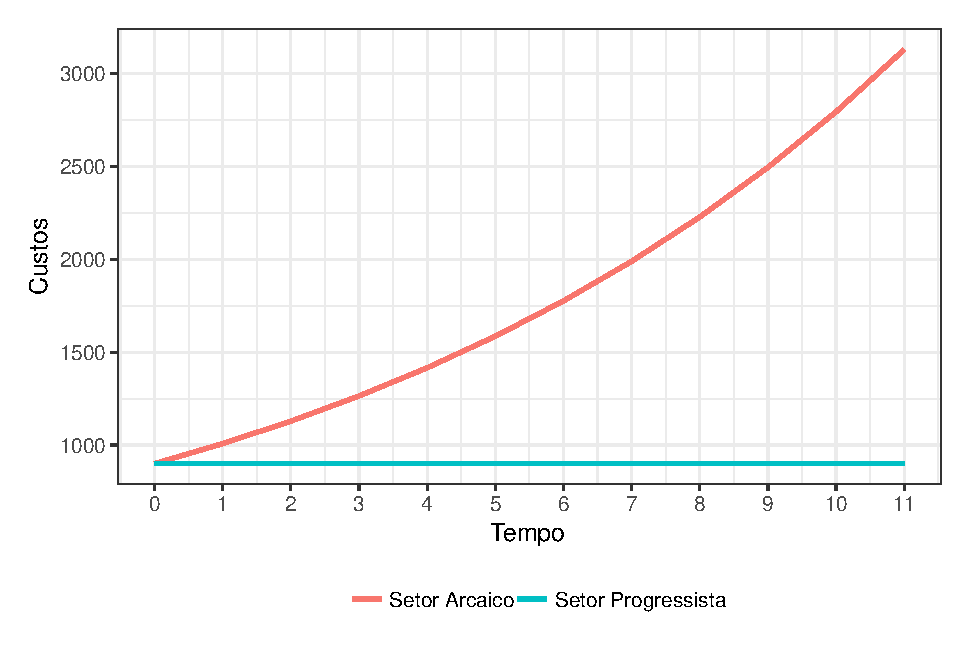
\includegraphics[scale=1]{doenca_dos_custos.eps}
		%	\fonte{Elaborated by the author.}
		%\end{figure}
		
		
		%\item ``A demanda de espetáculos ao vivo é elástica; toda alta de preço redunda numa redução do público'' \cite[p. 56]{benhamou2007economia}. Sendo os preços proporcionais aos custos relativos nos dois setores, $P_1 = \alpha C_1$ e $P_2 = \beta C_2$, então
		
		\item ``The demand of live shows is elastic; any price increase leads to a public reduction'' \cite[p. 56]{benhamou2007economia}. If the prices are proportional to the relative costs in both sectors, $P_1 = \alpha C_1$ and $P_2 = \beta C_2$, then
		
		$$\frac{P_1Y_1}{P_2Y_2} = \frac{\alpha C_1Y_1}{\beta C_2Y_2} = Cte$$ or
		$$\frac{C_1Y_1}{C_2Y_2} = \frac{W(1+r)^t \cdot L_{1,t}}{W(1+r)^t \cdot L_{2,t}} = \frac{L_{1,t}}{L_{2,t}} = K_0$$ and
		$$\frac{Y_1}{Y_2} = \frac{aL_{1,t}}{bL_{2,t}(1+r)^t} = \frac{aK_0}{b(1+r)^t}$$
		
		%``Quando \textit{t} aumenta, $\frac{Y_1}{Y_2}$ diminui, e quando $t \rightarrow \infty$, $\frac{Y_1}{Y_2} \rightarrow 0$'' \cite[p. 57]{benhamou2007economia}. Desse modo, a produção do setor arcaico (1) diminui fatalmente.
	%\end{enumerate}
	
	``When \textit{t} increases, $\frac{Y_1}{Y_2}$ decreases and when $t \rightarrow \infty$, $\frac{Y_1}{Y_2} \rightarrow 0$'' \cite[p. 57]{benhamou2007economia}. Thus, production in the archaic sector fatally descreases.
	
	\end{enumerate}
	%De forma complementar à lei de Baumol, \citeonline{throsby1994production} desenvolve uma função da produção do espetáculo ao vivo a qual pode ser sintetizada da seguinte forma:
	
	Complementarily to Baumol's law, \citeonline{throsby1994production} develops a function of live performance production which can be synthesized in this way:
	
	%O número de representações de uma determinada temporada deve ser fixado levando em conta a capacidade da sala \textit{v}. Sejam $L^s$ e $K^s$ o trabalho e o capital necessários para montar uma produção, sejam $L^r$ e $K^r$ o trabalho e o capital requeridos por cada representação da produção, o número de espectadores da iésima representação da jésima produção, $y_{ij}$, tal que $y_{ij} \leq v$, é dado por
	
	The number os presentations in a given season must be fixed taking into account the capacity of the auditorium \textit{v}. Be $L^s$ and $K^s$ the necessary work and capital to a production, be $L^r$ and $K^r$ the work and capital required by each performance of the production, the number of spectators of the performance \textit{i} of the production \textit{j}, $y_{ij}$, such that $y_{ij} \leq v$, is given by
	$$y_j = \sum_iy_{ij} = y_i(L^{s}_{j}, K^{s}_{j}, m_j, q_j) $$ where
	%o número de representações da jésima produção $$m_j = m_j(L^{r}_{j}, K^{r}_{j})$$ e $q_j$ resume as qualidades da jésima produção as quais, nesse contexto, podem ser medidas pela luxuosidade (\textit{lavishness}) da produção. Nesse caso, $q_j$ não é independente de $L^s$ e $K^s$. Espera-se que $$\frac{\partial y_j}{\partial m_j} > 0 \quad, \quad \frac{\partial^2y_j}{\partial m^{2}_{j}} < 0,$$ isto é, extender a temporada pode reduzir o número de espectadores na margem.
	
	the number of performances of the production \textit{j} $$m_j = m_j(L^{r}_{j}, K^{r}_{j})$$ and $q_j$ summarizes the qualities of the production \textit{j} which, in this context, can be measured by the lavishness of the production. In this case, $q_j$ is not independent of $L^s$ and $K^s$. It is expected that $$\frac{\partial y_j}{\partial m_j} > 0 \quad, \quad \frac{\partial^2y_j}{\partial m^{2}_{j}} < 0,$$ that is, extend the season can decrease the spectators number in the margin.
	
	%Segundo \citeonline[p. 59]{benhamou2007economia} ``a conclusão do modelo [de Baumol] é a inelutabilidade do aumento dos déficits dos espetáculos ao vivo''. Esse modelo tem sido corroborado por várias pesquisas \cite[e.g.]{throsby1979economics,leroy1980economie,peacock1983inflation,baumol1984inflation,dias2011artes} e, para \citeonline[p. 54]{benhamou2007economia}, essa característica do setor é suficiente para justificar o aumento das subvenções públicas e da prática do mecenato mesmo tendo em vista que ``essa intervenção maciça, distribuída de forma muito desigual, não é suficiente para garantir ao setor um equilíbrio financeiro duradouro''. Para \apudonline[p. 320]{baumol1966performing}{luksetich2011orchestras}, ``se se concorda que a artes de performance conferem benefícios gerais à comunidade como um todo\ldots as artes são bens públicos cujos benefícios demonstravelmente excedem as receitas que se espera coletar na bilheteria\footnote{If one agrees that the performing arts confer general benefits on the community as a whole\ldots the arts are public goods whose benefits demonstrably exceed the receipts one can hope to collect at the box office.}''. O modelo, entretanto, possui inconsistências, algumas delas apontadas por \citeonline{benhamou2007economia}.
	
	According to \citeonline[p. 59]{benhamou2007economia} ``the conclusion of Baumol's model is the ineluctability of the increase on deficit of live performance''. This model has been corroborated by many researches \cite[e.g.]{throsby1979economics,leroy1980economie,peacock1983inflation,baumol1984inflation,dias2011artes} and, to \citeonline[p. 54]{benhamou2007economia}, this sector characteristic is suficient to justify the increase of public subsidies and the practice of patronage even in view of the fact that ``this massive intervention, distributed in a very unequal way, is not enough to ensure to the sector a lasting financial equilibrium''. To \apudonline[p. 320]{baumol1966performing}{luksetich2011orchestras}, ``if one agrees that the performing arts confer general benefits on the community as a whole\ldots the arts are public goods whose benefits demonstrably exceed the receipts one can hope to collect at the box office''. 
	
	%%% Será que eu continuo este pedaço aqui????????????????
	
	%The model, however, has inconsistencies, some of them pointed by \citeonline{benhamou2007economia}.
	
	%A primeira consiste do pressuposto de que os salários do setor 1 são iguais aos do setor 2. Entretanto, desde a Segunda Guerra Mundial, os salários médios no setor do espetáculo ao vivo apresentaram uma tendência a crescerem menos do que no outro setor \apud{throsby1994production}{benhamou2007economia}. A segunda consiste do pressuposto altamente discutível de que a demanda é sensível ao preço. Maior parece ser o efeito da qualidade (percebida) do espetáculo sobre a demanda. De fato, \citeonline{throsby1994production} salienta que, por causa da dificuldade na medição da qualidade das performances, os efeitos dessa variável usualmente ficam restritos ao termo do erro nos modelos econométricos com a exceção de um estudo experimental conduzido pelo próprio \citeonline{throsby1983quality}. Nesse trabalho, o autor identificou algumas características da qualidade da performance no teatro como a qualidade da atuação, da produção, do roteiro e encontrou que a demanda é inelástica com relação ao preço dos ingressos mas \textit{altamente correlacionada com a qualidade esperada}. Este ponto parece central na investigação do mercado das orquestras e será desenvolvido oportunamente.
	
	
	
	%Além disso, é possível reduzir os custos de uma produção de espetáculo ao vivo de várias formas, a saber, através da gravação e reprodução do espetáculo, através do uso, na música, de sons \textit{sampleados} ou eletrônicos ao invés da contratação de músicos, a utilização de um mesmo ator representando mais de um papel em uma montagem cênica ou a reutilização de cenários e figurinos (práticas comum em montagens modernas de ópera), dentre várias outras. Para \citeonline[p. 60]{benhamou2007economia} esses meios ``equivalem a substituir o déficit comercial por um `déficit artístico'. Mesmo assim, essas medidas não são suficientes para compensar a diferença de produtividade. 
	
	%A terceira inconsistência reside no fato de que a alta da produtividade nos setores progressistas acompanhada por um aumento de salário proporcional à melhora das qualificações provoca um crescimento da procura por espetáculos, o que \textit{per se} contribui com a solução das dificuldades criadas pela diferença de produtividade nos setores \apud{throsby1979economics}{benhamou2007economia}. O crescimento, para \apudonline{baumol1966performing}{benhamou2007economia} reside na presença de consumidores cada vez mais sagazes e exigentes e acaba por gerar custos marginais superiores às receitas. ``As companhias musicais ajudaram a construir a reputação de artistas cuja contratação se tornou inevitável. A consequência é um aumento exagerado dos cachês e dos custos'' \cite[p. 61]{benhamou2007economia}. 
	
	%Por mais que seja verdadeira esta última constatação sobre os custos gerados na contratação de artistas de renome, parece também uma grande ingenuidade acreditar que o aumento de salário acarreta um crescimento na procura por espetáculos ao vivo. Na verdade os estudos em sociologia econômica tem mostrado, como veremos, que o consumo artístico está ligado ao que Bourdieu (\citeyear{bourdieu2011forms,bourdieu2003amor,bourdieu2007distincao}) chama de ``capital cultural'' e à construção de uma identidade social. 
	
	%A quarta inconsistência é esta: A gravação dos espetáculos pode gerar receita. Embora as rendas de espetáculos gravados sejam pequenas conforme investigações no contexto americano \apud{heilbrun2001economics}{benhamou2007economia} parecem ser um recurso bastante explorado no setor Algumas orquestras brasileiras costumam disponibilizar as gravações de seus concertos e óperas como produto secundário da sua carta de produtos. Gravações de estúdio e ainda outros produtos (camisetas, acessórios, \textit{souvenirs}) compõem o financiamento dessas instituições. Oportunamente abordaremos esse ponto.
	
	%\citeonline{throsby1994production}, após revisar vários estudos que testam a lei de Baumol conclui que
	
	%\begin{citacao}
		%Os impactos combinados dos ajustes de produção aumentaram a demanda e níveis crescentes de receita não esperada contrariaram qualquer tendência em direção a um aumento secular nos déficits entre companias de performance sugerindo que, embora a doença dos custos irá indubitavelmente continuar a presentear a artes performáticas com problemas difíceis, é improvável que chegue ao extremo\footnote{the combined impacts of production adjustments increased demand, and generally rising levels of unearned revenue have countered any tendency towards a secular rise in deficits among performance companies, suggesting that although the cost disease will doubtless continue to present the performing arts with difficult problems, it is unlikely to be terminal.}. \cite[p. 16]{throsby1994production}
	%\end{citacao}
	
	%Por fim, a análise de \citeonline{baumol1966performing} apontando a especificidade do setor contribuiu tanto para o desenvolvimento do programa de pesquisa que hoje conhecemos como economia da cultura quanto para o reconhecimento da necessidade de vinculação dos espetáculos ao vivo à esfera não-comercial subvencionada. Sigamos agora examinando como o mercado cultural brasileiro obtém seus recursos e o principal mecanismo de financiamento para que isso aconteça: as leis de incentivo à cultura.
	
	Baumol's analysis pointing the specificities of the cultural sector contributed to both the development of the research program that we know today as economy of culture and the recognition of the necessity of binding live performances to the subsidized non-commercial sphere. However, this approach is a standard economic one which, for the purposes of this investigation, lacks some of the social elements that are important to understand the shaping of a market, namely, institutions, social control, cooperation and social coordination, etc. Therefore, we will now try to build a theoretical framework inside social theory and accounting for the findings we have seen so far. Let us start presenting each of the elements we are going to aggregate in our analysis framework, namely, (1), White's $W(y)$ model, (2), Fligstein's theory, (3), normative isomorphisms and (4) multilevel networks.
	
	
	\chapter{The Social Construction of Markets}
	
	%Para Harrison \citeonline{white2002markets}, os mercados não são dados mas são estruturas sociais que emergem de interações complexas de seus componentes. Essas interações podem acontecer tanto de forma competitiva quanto, argumentamos, de forma cooperativa visando estabilização do mercado e redução do que o professor White chama de ``incerteza knightiana\footnote{Em referência ao economista americano Frank H. Knight.}''.
	
	To Harrison \citeonline{white2002markets}, markets are not given but they are social structures that emerge from complex interactions between its components. This interactions can occur competitively and, we argue, cooperatively aiming the stabilization of the market and the reduction of what White calls ``knightian uncertainty''\footnote{In reference to the american economist Frank H. Knight.}
	
	%Sua teoria visa explicar ``como as firmas minimizam incertezas formando um mercado como uma coleção de nichos baseada em sinais observados em seus engajamentos\footnote{(...) how firms minimize uncertanty by forming a market as a collection of niches based on signals observed in their commitments.}'' \cite[p. xiii]{white2002markets}. Em que consiste, portanto, um mercado de produção? A resposta para essa pergunta perpassa duas dimensões. A primeira, já comentada no parágrafo acima, remonta à natureza interdependente de sua estrutura, ou seja, uma emergência a partir das dependências de seus próprios fluxos. A segunda remonta ao seu mecanismo de operação o qual consiste dos engajamentos das diversas firmas em fluxos de produtos nos quais a procura do comprador agregado foi incorporada. Para esse autor ``Os fluxos resultantes de bens ou serviços diferenciados do mercado se dividem entre diversos compradores como opções igualmente boas: \textbf{a disciplina do mercado está centrada na qualidade do produto}\footnote{Resulting streams of differentiated goods or services from the market get split among diverse buyers as equally good options: The market discipline centers on product quality.}'' \cite[p. 1, grifo meu]{white2002markets}. Este ponto é central na caracterização de nosso objeto de estudo. O que seriam, entretanto, disciplinas de mercado?
	
	White's theory aims to explain ``how firms minimize uncertanty by forming a market as a collection of niches based on signals observed in their commitments'' \cite[p. xiii]{white2002markets}. What is a production market? The answer to this question goes through two dimensions. The first relates to the independent nature of its structure, that is, an emergence from dependencies on its own flows. The second concerns its operation mechanism which consists of commits by several firms in product flows in which the demand of the aggregate buyer was incorporated. To \citeonline[p. 1]{white2002markets} ``Resulting streams of differentiated goods or services from the market get split among diverse buyers as equally good options: The market discipline centers on product quality''. This is a central point in our study object's description. But first, what would be market disciplines?
	
	%\citeonline[p. 63]{white2008} indica que ``disciplinas oferecem regras dos jogos que produzem coordenação em tarefas em um mundo que, do contrário, seria caótico\footnote{Disciplines offer rules of the games that yield coordination in tasks in an otherwise messy world.}''. As disciplinas permitem ações conjuntas dando ordem aos laços traçados entre identidades em rede. Cada disciplina possui um tipo de processo que agrega a ação conjunta. Elas possuem ainda um ordenamento de valor específico pelo qual a estrutura se organiza hierarquicamente (por isso, podemos entender as disciplinas também como um sistema local de status). Dentre os tipos ideais de disciplinas elencadas pelo autor, aquela que se aplica aos mercados é chamada de \textit{interface}. Seu processo típico é o \textit{engajamento} que gera fluxos produtivos. O valor distintivo típico desse tipo de disciplina é a \textit{qualidade}.
	
	\citeonline[p. 63]{white2008} indicates that ``Disciplines offer rules of the games that yield coordination in tasks in an otherwise messy world''. Disciplines allow joint action giving order to ties between identities in a network. Each discipline has a type of process that aggregates joint action. They have also an order of a specifical value by which the struture is hierarchically organized (therefore, we can also understand disciplines as a local status system). Among ideal types of disciplines, the one which applies the best to markets is called \textit{interface}. Its typical process is the \textit{commit} that generates productive flows. The typical distinctive value of this discipline is \textit{quality}.
	
	%No caso dos mercados de produção, as firmas engajam fluxos de produtos direcionados ao comprador agregado que são percebidos na interface do mercado como igualmente bons. O distintivo social, o ordenador de valor nessa estrutura, é a qualidade.
	
	
	
	%Como se articulam os mercados? Para \citeonline{white2002markets}, algumas distinções básicas precisam ser feitas para entendermos sua estrutura. A primeira delas concerne a distinção entre \textit{downstream} e \textit{upstream}\footnote{Pela grande dificuldade em traduzir esses termos, optamos por mantê-los conforme o idioma original. Uma tentativa de tradução pouco elegante poderia ser feita como ``fluxos para baixo'' e ``fluxos para cima''.}, ou seja, os fluxos de produtos engajados pelo produtor em direção ao comprador agregado e a demanda desse comprador agregado o qual é incorporada nos produtos. Essa distinção gera uma segunda distinção concernente a três possíveis papeis para as firmas num mercado, a saber, fornecedor, produtor e comprador. Cada mercado possui uma orientação \textit{upstream} ou \textit{downstream}. Segundo o autor, ``os produtores não estão imbricados em um mercado, como o sociólogo Mark \citeonline{granovetter2007acao} argumentaria; eles de fato constituem a interface do mercado como um set de suas percepções e escolhas\footnote{Producers are not just embedded in a market, as the sociologist Mark Granovetter (1985) [na citação original] would argue; they actually constitute the market's interface in, and as the set of, their perceptions and choices.}'' \cite[p. 8]{white2002markets}. A constituição da interface do mercado se dá em direcionamento à origem percebida de risco. Nesse ponto, para White, reside a fraqueza da teoria econômica ortodoxa.
	
	
	
	%Ora, a teoria econômica ortodoxa oferece várias tentativas de modelagem de mercados empíricos/realísticos e, para isso, ancora-se em várias asserções provenientes do senso comum. Muito embora esse corpo de conhecimento possua modelos econométricos sofisticados, ele reside muito próximo do senso comum. Entretanto, ao abordar fluxos de produtos em rede num ambiente realístico, a teoria econômica ortodoxa abandona seus modelos, sejam eles realísticos ou de senso comum, e se atém à ficção da competição perfeita. Para \citeonline[p. 9]{white2002markets} ``um enorme custo dessa ortodoxia tem sido a infiltração desapercebida de noções de competição pura na pesquisa de economistas práticos\footnote{One great cost of this orthodoxy has been the unacknowledged infiltration of notions of pure competition into practical economists' research.}''. Do mesmo modo, a sociologia também tem relutado em incorporar os achados da teoria econômica em tentativas de construir críticas mais gerais à influência econômica nos processos sociais a partir das pesquisas de mercados específicos.
	
	How, then, can we undestand the statiblization of a markets interface? Which of its properties can collapse to the ``knightian uncertainty''?
	
	%Como, então, podemos entender a estabilização de uma interface de mercado? Que propriedades dela podem sucumbir à ``incerteza knightiana'' que atua contra seus membros?


	\section{Stabilizing the knightian uncertainty}
	
	%Transações num mercado tem mais a ver com interações repetitivas do que com momentos únicos. Desse modo, o volume de fluxos de produtos em um mercado pode funcionar como um sinalizador para os produtores sobre os engajamentos. Nas palavras de White:
	
	Market transactions have more to do with repetitive interactions than with unique moments. Thus, the volume of product flows in a market can function as a signal to producers about commits. White states that
	
	\begin{citacao}
		Each can orient to a niche by the size that is appropriate to the market's assessment of its quality compared to that of its fellows, who also are orienting to niches: the market as a joint social construction. \cite[p. 10]{white2002markets}
	\end{citacao}
	
	%Atrelado à interface do mercado está a noção de qualidade que, embora seja comumente tomada por uma característica inerente aos produtos, emerge das interações entre julgamentos tanto de produtores quanto de compradores. Desse modo,
	
	Attached to market's interface is the notion of \textit{quality}. Although it is commonly taken by an inherent characteristic of the products, it emerges from interactions between producers and buyers judgements. Thus, 
	
	\begin{citacao}
	(\dots) it is dual notions of differential quality, referent both to product and to producer, that become established as the core around which a set of market footings for producers can reproduce itself as footings in a joint market profile. The two sides, buyers and producers, exert contending pressures on the shape of this profile, pressures that correlate with their respective discriminations of quality. \cite[p. 10]{white2002markets}
	\end{citacao}
	
	%Cada produtor busca diferenciar seu produto e ao mesmo tempo reconhece um sistema de diferenciação  -- o índice de qualidade -- para sua versão de um produto no mercado. Nesse contexto, as escolhas interagem com influência e calibram os engajamentos repetidos de fluxos de produção e de pagamentos. Essa interação entre escolhas pressupõe um mínimo de comparabilidade o que é obtido de uma forma mais simples numa ordem linear de precedência. ``A reputação num ordenamento individual é a moeda de disciplina para mercados de produção'' \cite[p. 10]{white2002markets}, o que se torna difícil de sustentar com muitos participantes devido às nossas limitações cognitivas e de percepção. 
	
	Each producer seeks to differentiate his product and, at the same time, he recognizes the differentiation system -- the quality index -- to his version of a market product. In this context, choices interact with influence and calibrate the repeated commits of production flows and payments. This interactions between choices pressuposes a minimum of comparability which is obtained in a much simpler way in a linear order of precedence.
	
	\section{The mechanism behind production}
	
	%Os engajamentos de fluxos de produtos estão alinhados, de acordo com \citeonline[p. 12]{white2002markets}, a nove fenômenos. São eles:
	
	According to \citeonline[p. 12]{white2002markets}, flow commits are related to various phenomena, some of them specially interesting to our modelling rationale:
	
	\begin{enumerate}
		%\item um \textit{pequeno número} reconhecido de firmas que constituem uma linha negócios;
		\item a \textit{small number} of recognized firms that constitute a business line;
		%\item um ordenamento \textit{desigual} entre firmas incluindo sua distribuição de lucros e volume de fluxos de produtos engajados no mercado;
		\item an unequal ranking between firms including their profit distribution and product commits in the market;
		%\item as firmas visam \textit{lucro} e não se engajam, conforme a teoria econômica ortodoxa, em um sistema de ``soma zero'';
		\item firms aim \textit{profit} and do not commit, as orthodox economic theory states, to a \textit{zero sum system};
		%\item se as condições permitem o aumento da produção, espera-se que o custo unitário diminua gerando \textit{maiores retornos};
		\item if conditions allow the production raise, one would expect that unitary cost diminishes generating (bigger return);
		%\item em algumas linhas de negócios, reconhecimento de qualidade superior de um produto exige custos estruturais menores do que outros produtos de qualidade reconhecidamente inferior gerando \textit{retornos perversos};
		\item in some business lines, the recognition of a superior quality product demands smaller structural costs than other products with acknowledged inferior quality;
		%\item \textit{monopólios} são fenômenos extremamente \textit{raros};
		\item \textit{monopolies} are extremely \textit{rare};
	\end{enumerate}
	
	%Esses fenômenos são explicáveis entre si e atravessados por um modelo operacionalizado segundo parâmetros específicos. Nos deteremos agora nesse modelo desenvolvido por \citeonline{white2002markets}.
	
	%We will now focus on the model developed by \citeonline{white2002markets}.
	
	%O modelo parte do pressuposto fundamental de que qualidade e identidade não emanam um do outro mas produzem um ao outro nas interações entre as firmas num mercado. A qualidade é aqui entendida como uma construção social e não como um atributo evidente.

	These phenomena are crossed by an operationalized model which we will present now. The model makes a fundamental assumption that quality and identity are not build one from the other but produce each other inside firm interaction in a market. Quality is understood here as a social construction, not like an evident attribute.
	
	\section{Whites production model}
	
		%Chamemos o retorno total recebido por um volume de produtos de \textit{valor} (\textit{worth}). Seja  $W(y)$ o valor do volume $y$. Basicamente, o perfil do mercado pode ser inferido a partir da observação do comportamento dos pares volume-valor (Figura \ref{white_1.2}). 
	
	Let us call \textit{worth} the total revenue $W(y(k))$ of the \textit{volume} $y(k)$ sold by each firm $k$. This can be approximated in a continuos function $W(y)$. Basically, the Market Profile -- or Market Schedule -- can be inferred from the observation of pairs volume-worth behaviour (cf. Figure \ref{white_1.2}). 
	
	
	\begin{figure}[ht]
		\centering
		\caption{A profile market}
		\label{white_1.2}
		\includegraphics[scale=1]{white_1_2.png}
		\fonte{Adapted from \citeonline[p. 15]{white2002markets}}
	\end{figure}
	
	Each firm $k$ tries to select the optimum $y(k)$ and also adjust its \textit{price} strategy 
	$ W(y(k))/y(k) = p(y(k)) $
	to maximize \textit{profit}
	$ W(y) - C(y(k), k) $. Therefore, \citeonline[p. 36]{white2002markets} states the cost schedule for the variation of a producer's cost with volume as
	
	\begin{equation}
	\label{cost}
		C(y, n) = q \cdot y^c \cdot n^d
	\end{equation}
	
	where the two main parameters are the exponents $c$ and $d$, expressions of elasticities. In this formula, $q$ is a numerical scaling factor across all the firms, a constant, $y$ represents the volume of product commitment and $n$ is a quality component, the very identity of the product of that firm. The $d$ parameter is specially interesting in this case. It will be analysed in more depth later.
	
	On the consumer's side, the aggregate buyer's \textit{satisfaction} $ S(y, n) $ is defined by 
	\begin{equation}
	\label{satisfaction}
		S(y, n) = r \cdot y^a \cdot n^b 	
	\end{equation}
		
	and it relies both on the number of units bought $y$ and on a \textit{qualitative component}, $n$. According to \citeonline{favereau2002markets}, since ``buyers in aggregate make a `yes or no' decision when offered a volume/price pair by a producer'', the only producers who stand out are those whose offer satisfies the following constraint:
	
	\begin{equation}
	\label{S-theta}
		S(y[n], n) = \theta \cdot W(y[n])	
	\end{equation}

	
	``The parameter $\theta$ is a sort of mark-up of satisfaction (\dots) over the overall buying cost of a given production'' \cite[p. 217]{favereau2002markets}. It is a ratio that functions as a ``deal criterion'' \cite[p. 39]{white2002markets}. The cost $C$ and the market schedule $W(y)$ are known by the producer but not the satisfaction function $S$ which are constructs of the observer.
	
	%A curva da figura \ref{white_1.2} é facilmente estimada por um analista de negócios como um guia para um perfil adequado dentro desse mercado. Esse perfil disciplina os engajamentos de cada firma quanto ao volume visando um resultado ótimo de Retornos X Custos. A qualidade se vê refletida nesse perfil e isso se dá sem a necessidade de um índice explícito. As definições da vida são incorporadas em um ordenamento de qualidade o qual perpassa o discurso vigente num domínio em rede. Esse ordenamento que condiciona a formação de laços na rede é percebido em termos de prestígio e combina qualidade de consumo e relações de concorrência \cite{white2002markets}.
	
	%Os esforços de uma firma refletidos em sua estrutura de custos tendem a ser refletidas em avaliações do comprador agregado. Essa correlação provê uma base para o ordenamento da qualidade percebida, a saber, um ordenamento linear suficiente para embasar o perfil do mercado. Mas qual é a relação entre os volumes engajados e a qualidade percebida? Isso depende da linha de negócio.
	
	The efforts of a firm embedded in its cost structure tend to be reflected in the aggregate buyer evaluations. This correlation provides a base for the perceived quality ranking, namely, a linear ordering sufficient to base market's profile. But what are the relations between commit volumes and the perceived quality? To White, that depends on the business line. \citeonline{white2002markets} explains that
	
	%\citeonline{white2002markets} explica, tirando o foco da empresa que atua como compradora e depositando no comprador final -- indivíduo -- e sua percepção de qualidade, que:
	
	\begin{citacao}
		Sometimes, a large $y$ connotes higher quality, as in the soda pop industry, but at other times, lower quality, as in the wine industry. So the frequency with which buyers encounter a producer's output (\dots) can signal different things across different shapes of profile. As some goods monopolize shelf space, wealthier suburban mothers, like wealthy East Siders in Manhattan, shy away from them, since they are what the average person is buying. For other goods that receive high exposure in advertising, that's precisely what these shoppers buy. After all, the fact that everyone else is buying it confirms that it's the best. \cite[p. 15]{white2002markets}
	\end{citacao}
	
	%O ordenamento da qualidade, portanto, envolve um contexto social onde as empresas possuem uma distribuição prévia de prestígio que mescla sua reputação com a de seus produtos. Fluxos de informação são centrais no mecanismo de reprodução de um mercado de produção. Informação útil ao produtor, entretanto, não precisa coincidir com a informação formulada por outros. ``Quando possível para os atores usarem informações lidas das ações de outras, chamamos essa informação de \textit{sinal}. Engajamentos anteriormente feitos são em si mesmos sinais lidos como perfil pelos produtores\footnote{When it is possible for actors to make use of information read from the doings of others, let's call this information a \textit{signal}. Fulfilled prior commitments are themselves the signals read off as profile by the producers.}'' \cite[p. 16]{white2002markets}.
	
	In this sense, the quality ranking involves, therefore, a social context where firms have a previous prestige distribution that mixes their reputation with the reputation of their products. ``When it is possible for actors to make use of information read from the doings of others, let's call this information a \textit{signal}. Fulfilled prior commitments are themselves the signals read off as profile by the producers'' \cite[p. 16]{white2002markets}. Thus, the author defines market production mechanism in this way:
	%White resume o mecanismo dos mercados de produção da seguinte maneira:
	
	\begin{citacao}
		A production market forms around and thus consists in a joint interface between producers confronting uncertainty from the other side of the interface. This interface is energized by rivalry among its peer producers, all seeking buyers for their continuing streams of production in amounts optimal for their individual cost structures. The producers have come to signal each other through a profile across their production commitments. \cite[p. 27]{white2002markets}
	\end{citacao}
	
	Let us now take a closer look to the elasticities parameters, the exponents $a$, $b$, $c$ and $d$, to understand how the market can be understood in terms of these variables.
	
	\section{The topology of markets -- elasticities parameters}
	
	To \citeonline{white2002markets}, the four elasticities parameters, saturation terms that shape the market curves, when analyzed jointly allow for the investigation of the viability of the market. Parameters $b$ and $d$ are measures of dispersion across quality, ``the exponents of discount of valuation with declining quality by, respectively, taste of consumers and cost of producers'' \cite[p. 50]{white2002markets}. The same way, $a$ and $c$ are saturation parameters for volume produced. These parameters relate themselves as we describe in table \ref{exponents-abcd}.
	
	\begin{table}[ht]
		\ibgetab{
		\caption{Tabulation of parameters}
		\centering
		\label{exponents-abcd}
	}
	{\begin{tabular}{l c c}
			\hline
			\hline
			   					& \textit{Buyer Need} & \textit{Producer Cost} \\
			\hline
			Volume sensitivity	& a					  & c						\\
			Quality sensitivity	& b					  & d						\\
			\hline			
		\end{tabular}
	}
	{\fonte{\cite[p. 51]{white2002markets}}}
	\end{table}
		
	
	According to \citeonline{white2002markets}, we should combine the parameters in ratios in a way that each ratio with buyer side in the numerator and producer side on the denominator makes an axis of the market plane. This allows for a simplified representation of the possible market profiles despite of the complexity of the $W(y)$ model (cf. FIG. \ref{market-plane}).
	
	
	\begin{figure}[th]
		\centering
		\caption{Market plane, designating four regions, three locations}
		\label{market-plane}
		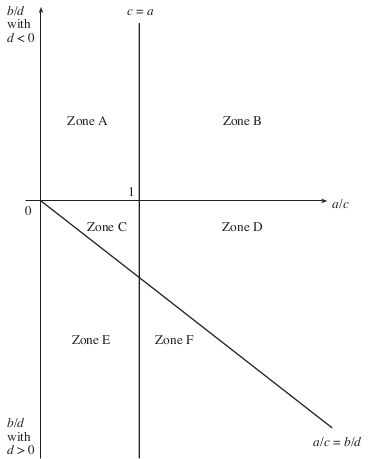
\includegraphics[scale=1]{market_plane_favereau.png}
		\fonte{\cite[p. 229]{favereau2002markets}}
	\end{figure}

	To \citeonline{eloire2009reseaux}, the main goal of White's model is to show the structure of the market. The market plane shows six zones; four of them are zones that demarcate viable market, the other two, non-viable or unraveling. They can be described in a simplified way\footnote{A mathematical development of this plane is described in Appendix 1.} like this:
	
	Zone C is labelled \textbf{ordinary}. In this zone, revenues decrease to scale ($a/c < 1$) since cost increases with quality ($d > 0$). This is the `ordinary' that we think about quality. Also, returns are decreasing to quality to a more severe degree than to scale ($a/c > b/d$). Zones D and F are labelled \textbf{advanced}. In this zone higher quality is more expensive to produce ($d > 0$) and revenues increase to scale ($a/c > 1$). Zone A is labelled \textbf{paradox}. In this zone, in contrast with the ordinary thinking, higher quality is less costly to produce than lower quality ($d < 0$) although there are decreasing returns to scale ($a/c < 1$). B and E are non-viable market zones. 
	
	\section{Measurements}
	
	In the $W(y)$ model, measurements are an issue to be solved in a creative way because White does not close the scope of the variables to be chosen. The review of two important studies gives us a basis to decide on this measurement issue.
	
	\citeonline{biencourt2002market} studied the theatrical institutions markets. They argue that the main advantage of White's model is related to the interdependence of the market structure and individual decisions through niches. This is particularly interesting to this specific case because
	
	\begin{citacao}
		Theatrical organizations base their construction of niches on the competencies of their administrative, technical and artistic teams, the public's former experiences and the programming policy that orients choices of repertories and directors. The concept of a niche is suited to the uniqueness of performances. Their quality is the result of a combination of the quality of actors' and technicians' individual work on a project, under the control of the director. \cite[p. 255]{biencourt2002market}
	\end{citacao}
	
	
	If we retake the functions of satisfaction (\ref{satisfaction}) and cost (\ref{cost}), the variables were chosen in this manner:
	
	\begin{itemize}
		\item \textbf{Volume of production $Y$} -- estimated by number of performances listed in the theaters' annual report.
	\end{itemize}

	The authors show that for \apudonline{throsby1993economics}{biencourt2002market} the number of tickets sold is a better suited indicator for $Y$. However, ``the determination of $S$ would then require one to know the degree of audience satisfaction after each performance, something that is impossible'' \cite[p. 264]{biencourt2002market}. The number of seats available for each performance would also have been a good indicator if the authors had access to this data.
	
	\begin{itemize}
		\item \textbf{The satisfaction of consumers $S$} -- measured by the number of paid visitors to the institution market.
	\end{itemize}
	
	The authors justify this choice showing data from previous research on theatre audiences' habits and representations. Also, they divided the performances on four repertoire categories, namely, ``classical'', ``20th century'', ``contemporary French'' and ``contemporary foreign'' plays. They also make a correction for the repertory effect by ``multiplying the number of paying visitors observed  in each of the four categories by the average ratio $\bar{x}_i$ between the share of performances and that of the number of visitors in a given genre $i$ for all the institution markets'' \cite[p. 265]{biencourt2002market}. Let $\tilde{P}_i$ be the number of performances and $\tilde{V}_i$ be the number of paying visitors to all theatres in category $i$. The average can be defined by
	
	\begin{equation}
	\label{repertory-effect-correction}
		\bar{x}_i = \frac{\tilde{P}_i / \sum_{i=1}^{4}\tilde{P}_i}{\tilde{V}_i / \sum_{i=1}^{4}\tilde{V}_i}	
	\end{equation}
	
	If $v_i$ represents the number of paying visitors in category $i$ of repertoire, the public satisfaction can be estimated by
	
	\begin{equation}
	\label{satisfaction-corrected}
		S = \sum_{i=1}^{4}\bar{x}_i v_i
	\end{equation}
	
	
	
	\begin{itemize}
		\item \textbf{The aggregated cost $C$} -- this variable was obtained by adding up theatrical artistic expenses (differentiated from fixed costs).
		
		\item \textbf{scale $r$} -- equal the inverse of the average price of seats $\bar{p}$ in all theatres.
		
		\item \textbf{scale $q$} -- considered equal to 1.
	\end{itemize}



        Although White's model represents a big step in the construction of knowledge about the markets, it has an issue related to its very core, the quality ranking. To him, quality is given in a predetermined social space. In fact, \citeonline{favereau2002markets} states that to agree on price is not a big deal but to agree on quality is intrinsically a problem. We shall argue, however, that quality is not predefined but actors struggle and negotiate on a daily basis for its definition.

        According to \citeonline{eloire2009reseaux}, by embracing the annual publications previously mentioned, this industry has ``specific judgement devices on quality'' as \citeonline{karpik2009elements}  argues. This devices do not only help the coordination between offer and demand, but they also ``contribuent au classement des producteurs selon des critères de qualité collectivement définis et surtout acceptés, mais qui sont aussi des objets de lutte pour leur définition'' \cite[p. 494]{eloire2009reseaux}. In fact, \citeonline{eloire2009reseaux} states that the very existence of various guides is, by itself, an evidence of this symbolic struggles for the definition of quality, although in the ``high distinction'' the guides seem to converge.

        What if there are no guides or websites to testify on orchestra's quality and the critics in the main newspapers in town are nearly nonexistent? Well, this is the case in Belo Horizonte and it poses a quite of a challenge. All the cultural economics and singularities economics discussion on quality relies on the action of critics who are, per excellence, the ones who have the primacy of quality definition. In Belo Horizonte, orchestral performances almost never get a critic and there is not such a well structured platform for it as Rotten Tomatoes\footnote{\url{https://www.rottentomatoes.com}.} or \textit{Adoro Cinema}\footnote{A famous Brazilian movie critics website. Available in \url{http://www.adorocinema.com}.} for movies. If critics do not act much within the field of our study object, where does the quality definition come from?
        
	\citeonline{biencourt2002market} present an interesting approach to the quality problem regarding theatres' market. We shall depart from their rationale to build the quality index $n$ we will use in this investigation.

        To deal with quality index $N$, the authors elaborate a sophisticated construct to explain how various actors have a different influence on quality. To them,
	
	\begin{equation}
	\label{biencourt-quality}
		N_{l}^{b_l} = N_{1l}^{b_{1l}} N_{2l}^{b_{2l}} N_{3l}^{b_{3l}} N_{4l}^{b_{4l}} 
	\end{equation}
	
	that is, the \textit{overall quality} $N$ in the year $l$ is constructed aggregating the judgements of \textit{drama critics} $N_1$, the judegements of \textit{programme planners} $N_2$, the judgement of the \textit{public authorities} $N_3$ and the influence of \textit{previous consumption} $N_4$. Now, each of these parts of the overall quality were measured in this manner:
	
	
	\begin{itemize}
		\item \textbf{Judgements of drama critics $N_1$} -- measured recording all reviews of shows scheduled in the theatres in \textit{Le Monde} and \textit{Libération} newspapers and \textit{Télérama} magazine, opinion leaders among drama critics.
		
		\item \textbf{Judgements of programme planners $N_2$} -- the normed ``indegree'' centrality of the theatre; in that case, this means the number of performances of shows produced by other theatrical institutions, scheduled by the theatre divided by the maximum centrality of the network.
		
		\item \textbf{Judgement of public authorities $N_3$} -- measured by the amount of state subsidies. To \citeonline[p. 267]{biencourt2002market}, ``this choice is justified by the weight of the state, which is greater that that of local authorities in the political recognition of an institution's artistic reputation''.
		
		\item \textbf{Influence of previous consumption $N_4$} -- measured by the number of paying visitors in the preceding period.
	\end{itemize}
	
	The overall quality perceived by the public is constructed by aggregating these four variables in the form of a Cobb-Douglas function (cf. equation \ref{biencourt-quality}). To measure the weight of each one of these variables on the overall quality, they estimated a linear model that had the number of paying visitors per performance as the dependent variable. Knowing that $r = 1/\bar{p}$ and taking into account equations (\ref{satisfaction}) and (\ref{biencourt-quality}), we can derive
	
	\begin{equation}
	\label{biencourt-derivation}
		[S\bar{p}/Y]_l = Y_{l}^{\hat{a}_l} N_{l}^{\hat{b}_l} \varepsilon_l = Y_{l}^{\hat{a}_l} N_{1l}^{\hat{b}_{1l}} N_{2l}^{\hat{b}_{2l}} N_{3l}^{\hat{b}_{3l}} N_{4l}^{\hat{b}_{4l}} \varepsilon_l
	\end{equation}
	
	where $l$ is the year under investigation. This leads to the linear model
	
	\begin{equation}
	\label{regression}
		\log([S\bar{p}/Y]_l) = \hat{a}_l \log Y_l + \hat{b}_{1l} \log N_{1l} + \hat{b}_{2l} \log N_{2l} + \hat{b}_{3l} \log N_{3l} + \hat{b}_{4l} \log N_{4l} + \hat{\varepsilon}_l
	\end{equation}
	
	From this, it is possible to deduce, without a constant,
	
	\begin{equation}
	\label{N-com-pesos}
		\log N_l = \hat{b}_{1l} \log N_{1l} + \hat{b}_{2l} \log N_{2l} + \hat{b}_{3l} \log N_{3l} + \hat{b}_{4l} \log N_{4l} + e_l \hat{\varepsilon}_l
	\end{equation}
	
	with $0 \le e_l \le 1$ assuming $\hat{b}_l = 1$.
	
	Then, the four elasticities exponents were deduced as solutions of a system of two equations to two unknowns. As the authors were studying two years seasons, by posing $\Delta = \log Y_l \cdot \log N_{l+1} - \log Y_{l+1} \cdot \log N_l$, they obtain:
	
	$$ a = \frac{ \log([S\bar{p}]_l) \cdot \log N_{l+1} - \log([S\bar{p}]_{l+1}) \cdot \log N_{l} }{\Delta} $$
	
	$$ b = \frac{ \log([S\bar{p}]_{l+1}) \cdot \log Y_{l} - \log([S\bar{p}]_{l}) \cdot \log Y_{l+1} }{\Delta} $$
	
	$$ c = \frac{ \log C_l \cdot \log N_{l+1} - \log C_{l+1} \cdot \log N_{l} }{\Delta} $$
	
	\begin{equation}
	\label{parameters}
		d = \frac{ \log C_l \cdot \log Y_{l+1} - \log C_{l+1} \cdot \log Y_{l} }{\Delta}
	\end{equation}
	



	% OBS: A partir da página 280, Éloire começar a falar dos niches de qualités e as variáveis que escolhe para medir cada parte do modelo.

	On the other hand, \citeonline{eloire2009reseaux} chose a different set of variables to measure the inputs of the $W(y)$ model. In his PhD thesis, he studied the market of restaurants in Lille. He also uses the number of clients as an indicator to $y$ and observes the revenues (\textit{Chiffre d'affaires}) as well as uses the average ticket price for $W$. In order to investigate the market plane, \citeonline{eloire2009reseaux} mobilized the variables described in Table \ref{eloire-abcd}:

        \begin{table}[ht]
        \ibgetab{
        	\centering
        	\caption{Quality niches parameters}
        	\label{eloire-abcd}
        }
         {\begin{tabular}{c | p{5cm} p{5cm}}
         		\hline
            & \textbf{Volume}  & \textbf{Quality} \\
            \hline
            \textbf{Satisfaction}  & \textbf{a} = Average number of clients per service & \textbf{b} = Average ticket value + Quality note \\
            \textbf{Cost} & \textbf{c} = Salaried / Couverts * Services & \textbf{d} = Ratio of salaried availability / clients \\
            \hline
          \end{tabular}
      	}
  		{\fonte{\citeonline[p. 289]{eloire2009reseaux}}}
        \end{table}

        % This here is on page 290!!!
	Éloire argues that quality is a social construction build between the offer from structured producers and an aggregated demand. In the restaurants case, it also depends on the ``cuisine'' style which is very difficult to measure. However, this culinary scale is closely correlated with simple economic statistics: price, availability ratio in a way that the higher the prices and the ratio, the more ``fancy'' is the restaurant. Therefore, he considers the quality cost (\textbf{d} parameter) is related to the availability ratio, that is the amount of personnel that a restaurant hires over the number of clients it intends to serve. Clients satisfaction (\textbf{b} parameter) can be represented by the average ticket value.

        % PAGE 290
        The author recognizes that the a restaurant's capacity is correlated to the volume of personnel. So, the volume costs (\textbf{c} parameter) are measured to the number of salaried employees divided by the (potential) number of cutlery multiplied by the number of services. Also, he acknowledges that a main strategy of the restaurants is related to the amount of time/time of the day that it stays open. Some restaurants can function 24/7, some only at lunch, some only at night,  and this implicates requires cost, personnel, logistics, etc. This is expressed on the \textbf{c} parameter calculus. The satisfaction at volume (\textbf{a} parameter) is measured by the average number of clients per service. This is derived of the restaurant's ``filling rate''. The higher this rate, the more we can infer that his decisions regarding volume costs are validated by the clients. On the other hand, the lower this rate, the more the volume costs can be seen as ``disproportional'' by the clients \cite{eloire2009reseaux}.

        The quality note pointed by the author in table \ref{eloire-abcd} is built aggregating the notes of five international restaurant guides, all of them well known and recognized in the profession, namely, ``Le Guide Michelin France'', ``Le Bottin Gourmand'', the ``GaultMillau'', the ``Champérard'' and ``Le Pudlo France''. The aggregation of these guides scoring was obtained through a specialized website\footnote{\url{http://restaurant-hitlisten.de/france/bewertung.htm}}.
        
	
	
         
        \subsection{Measuring the $W(y)$ model}

        NEEDS REVIEW!!!!!!!!!!!!!!!
        
        Let us recall the two main equations of the $W(y)$ model. First the Cost equation (\ref{cost}):
	$$C(y, n) = q \cdot y^c \cdot n^d$$
        then, the Satisfaction equation (\ref{satisfaction}):
        $$S(y, n) = r \cdot y^a \cdot n^b$$

        For the purposes of this investigation, the parameters will be measured in the following way:

        \begin{itemize}
        \item The constant $q = 1$;
        \item the constant $r =$ the inverse of the average price of seats in all performances of the season;
        \item The aggregated cost $C$ will be obtained by adding the orchestra's artistic expenses;
        \item The satisfaction of consumers $S$ will be estimated by a ratio of the number of paying individuals in the audience over the number of seats available;
        \item the volume of production $y$ will be estimated by the number of seats available for each performance\footnote{In case we cannot have access to data on the seats available, $y$ can be estimated by the total number of performances on a season.};
        \item the quality index $n$ will be estimated aggregating the ticket prices, total budget, ``closeness to the state'' note and the musicians perception;
        \end{itemize}

        We will also try to capture the audience quality perception through a web application that we will construct only for this purpose. We will compare the results generated by both $n$ measurements. We will discuss this web application in more detail in the next section.

        The elasticities $a$ and $b$, related to the Satisfaction equation, can be obtained as solutions of a system of two equations to two unknowns as it was proposed by \citeonline{biencourt2002market}. Trying to measure any of these variables would violate the assumption that cultural goods are not rivals in consumption.

        The elasticities $c$ and $d$, on the other hand, can be measured in the following way:
        % ELABORATE! ELABORATE! ELABORATE! ELABORATE! ELABORATE!

        \begin{itemize}
        \item $c =$ the number of salaried employees $/$ number of performances;
        \item $d =$ the total budget $/$ number of performances
        \end{itemize}

        This makes sense because....... % EXPLAIN!!!!!!!
	
	
	\section{Fligstein's model}
	
	
	%Neil \citeonline{fligstein2002architecture} traça uma teorização sobre a emergência e funcionamento dos mercados ligeiramente diferente da que vimos em White. Fligstein também leva em conta uma estrutura relacional onde firmas interagem entre si e com o comprador generalizado visando a estabilização do mercado (e consequente subsistência de todos). A grande diferença fica por conta da participação do Estado. Enquanto White não tece grandes considerações acerca do papel estatal na emergência e funcionamento dos mercados de produção, Fligstein elabora seu esquema teórico identificando a estrutura do Estado como central para o desenvolvimento dos mercados. Por que Estados? - pergunta Fligstein. O próprio autor responde que ``À medida que a possibilidade de padrões de interação complexos na esfera da troca econômica se expandem, os atores se mostraram incapazes de prover regras para si mesmos\footnote{As the possibility for complex patterns of interaction in the sphere of economic exchange has expanded, actors have proven incapable of providing rules for themselves.}'' \cite[p. 27-8]{fligstein2002architecture} e, portanto, recorrem ao Estado como provedor de regras para que o jogo econômico funcione de maneira justa.
	
	Neil \citeonline{fligstein2002architecture} builds a theory on the emergence and functioning of markets slightly different from White. Fligstein also takes into account a relational structure where firms interact with each other and with the generalized buyer seeking the stability of the market (and consequent subsistence of all). The main difference is about the role of the State. While White does not make major considerations on the role of the State on the emergence and regular functioning of production markets, Fligstein elaborates his theoretical scheme identifying the State structure as central to market development. Why States? - asks Fligstein. His answer is ``as the possibility for complex patterns of interaction in the sphere of economic exchange has expanded, actors have proven incapable of providing rules for themselves'' \cite[p. 27-8]{fligstein2002architecture} and therefore, they appeal to the State as a rule provider so the economic game can happen fairly.

        We will also argue that, beyond the State's role as the main market regulator, it is an active actor with a great weight in the definition of quality. It does so essentially by choosing which organization is going to receive funding and which is not, which organization will celebrate a partnership contract and which is not, etc.
	
	%\citeonline{fligstein2002architecture} concebe os mercados como ``campos'', arenas sociais onde vendedores e compradores se encontram. Essas arenas obedecem a quatro tipos puros de regras para a produção e reprodução de sua estrutura, quais sejam:
	
	\citeonline{fligstein2002architecture} conceives markets as ``fields'', social arenas where sellers and buyers meet. These arenas obey four pure types of rules for the production and reproduction of its structure:
	
	\begin{enumerate}
		\item property rights;
		\item governance structures;
		\item rules of exchange and
		\item conceptions of control.
	\end{enumerate}
	
	%Estas diferentes formas de regulação são inclusivas; o nível posterior necessariamente pressupõe o anterior. Do primeiro ao último há um maior grau de generalidade. 
	
		
	%Direitos de propriedade são, segundo o autor, regras que definem quem possui diretos sobre os retornos financeiros das firmas. Formas comuns de direito de propriedade são patentes e credenciais. Sua constituição não é, necessariamente, o desfecho de um processo eficiente mas um contínuo e contestável processo político \cite{fligstein2002architecture}.
	
	These forms of regulation are inclusive; the higher level necessarily contains the lower. Property rights are, according to Fligstein, rules that define who has rights over firms income. Common forms of property rights are patents and credentials. These rules are \textit{sine qua non} conditions of existence for markets since they define the relations between who has possession of some good and all the others. This stabilize markets. ``Property rights thus function to produce two forms of stability: defining the power relationships between constituencies in and around firms, and signaling to other firms who firms are'' \cite[p. 34]{fligstein2002architecture}.
	
	%Essa regras configuram condição \textit{sine qua non} de existência de mercados uma vez que definem as relações entre aqueles que detém posse de algum bem e os demais estabilizando o mercado. ``Os direitos de propriedade funcionam, portanto, para produzir duas formas de estabilidade: a definição de relações de poder entre constituintes dentro e fora das firmas e sinalizar a outros quem essas firmas são\footnote{Property rights thus function to produce two forms of stability: defining the power relationships between constituencies in and around firms, and signaling to other firms who firms are.}'' \cite[p. 34]{fligstein2002architecture}.
	
	%Estruturas de governança são estruturas de regras gerais ao nível da sociedade que definem relações competitivas e cooperativas entre firmas além de sua organização interna. Essas regras definem formas legais e ilegais de controle da competição no espaço mercantil. Elas podem aparecer na forma de leis (e.g., leis antitrustes) ou normas sociais muito embora assumam grande variação entre diferentes sociedades. Cabe ressaltar que a organização interna de uma firma também se dá como resposta a formas legais ou ilegais de competição no mercado. Firmas podem se integrar tanto verticalmente, como forma de assegurar seus insumos necessários, quanto horizontalmente, comprando ações visando produzir um ordenamento estável no mercado ou diversificando sua carta de produtos visando proteção contra os ``caprichos de produtos específicos'' \cite[p. 34]{fligstein2002architecture}. A formação de parcerias estáveis e de longo prazo também configuram respostas à competição.
	
	Governance structures are general rules on society level that define competitive and cooperative relations between firms and also their internal organizations. These rules define legal and ilegal forms of competition control in the market. They can be laws or social norms although they can assume great variability.
	
	
	%As regras de troca definem quem pode se engajar em transações comerciais com quem bem como suas condições. As regras abrangem pesos, padrões comuns, fretagem, cobrança, seguro, trocas financeiras e a firma de contratos. ``As regras de troca ajudam a estabilizar os mercados assegurando que as trocas ocorram sob condições que se aplicam a todos\footnote{Rules of exchange help stabilize markets by ensuring that exchanges occur under conditions that apply to everyone.}'' \cite[p. 35]{fligstein2002architecture}. Alguns dos tratados comerciais internacionais mais recentes como o GATT (\textit{General Agreement of Tariffs and Trade}) focam na harmonização das regras de troca.
	
	Exchange rules define who can engage in business transactions with whom as well as its conditions. Rules also apply to weights, common patterns, delivery, billing, insurance, financial trade and contract signing. ``Rules of exchange help stabilize markets by ensuring that exchanges occur under conditions that apply to everyone'' \cite[p. 35]{fligstein2002architecture}.
	
	%``Concepções de controle refletem acordos específicos de mercado entre atores em firmas sobre princípios de organização interna (\dots), táticas de competição ou cooperação (\dots), e a hierarquia ou o ordenamento de status das firmas num dado mercado\footnote{Conceptions of control reflect market-specific agreements between actors in firms on principles of internal organization (\dots), tactics for competition or cooperation (\dots), and the hierarchy or status ordering of firms in a given market.}'' \cite[p. 35]{fligstein2002architecture}. São, em sua essência, produtos histórico-culturais. São históricos à medida que se restringem ao contexto histórico de um determinado setor em uma determinada sociedade e são culturais pois formam um arcabouço de entendimentos e práticas vigentes num dado mercado. Para \citeonline{fligstein2002architecture}
	
	``Conceptions of control reflect market-specific agreements between actors in firms on principles of internal organization (\dots), tactics for competition or cooperation (\dots), and the hierarchy or status ordering of firms in a given market'' \cite[p. 35]{fligstein2002architecture}. They are, in their essence, cultural-historical byproducts.

	
	\begin{citacao}
		%Um mercado estável é um campo social no qual a concepção de controle define as relações sociais entre firmas vendedoras incumbentes e desafiantes de modo que as incumbentes reprodruzem essas relações de tempos em tempos. O propósito da ação em um dado mercado é criar e manter mundos estáveis dentro das firmas e entre elas que permita a sobrevivência de firmas dominantes\footnote{A stable market is a social field in which a conception of control defines the social relations between incumbent and challenger seller firms such that the incumbent firms reproduce those relations on a period-to-period basis. The purpose of action in a given market is to create and maintain stable worlds within and across firms that allow dominant seller firms to survive.}. \cite[p. 35]{fligstein2002architecture}
		A stable market is a social field in which a conception of control defines the social relations between incumbent and challenger seller firms such that the incumbent firms reproduce those relations on a period-to-period basis. The purpose of action in a given market is to create and maintain stable worlds within and across firms that allow dominant seller firms to survive. \cite[p. 35]{fligstein2002architecture}
	\end{citacao}
	
	%As concepções de controle evidenciam também, como podemos notar, um elemento político dos mercados no que toca à manutenção do ordenamento hierárquico vigente, sua reprodução e sua manifestação no processo de definição de padrões de qualidade e certificação. Dito de outra forma, as concepções de controle colocam perguntas como ``quem controla a entrada e saída de um sistema concorrencial?'' ``Como os desafiadores e os dominantes entram em relação?'' ``Quem consegue impor a pauta de qualidade num setor industrial, por exemplo, um \textit{standard} ISO ou um sistema de certificação do que é um produto orgânico no mercado de alimentos?''
	
	Conceptions of control evidence also a political element in markets regarding the maintenance of the current hierarchical order, its reproduction and its manifestation on the process of defining quality standards and certification. Conceptions of control lead to questions like ``who controls entrance and exit of a competitive system?'' or ``how challengers and dominants relate''?
	
	%Para Fligstein, a entrada de países em sistemas capitalistas ``empurra'' os Estados a uma posição regulatória com relação aos quatro tipos acima mencionados. No exercício regulatório, os Estados produzem normativas culturais que determinam o processo de estruturação da ação econômica. Esse exercício é contínuo. Constantemente os Estados lidam com situações de crise e com o \textit{lobby} das empresas clamando por intervenção estatal. Os rumos que os mercados tomam estão diretamente relacionados a dois fatores: (1) a capacidade de intervenção, regulação e mediação do Estado e (2) o poder de organizações privadas para influenciar os termos de intervenção.
	
	%O Estado tem ainda um papel fundamental no financiamento da inovação. Segundo \citeonline{fligstein2002architecture}
	
	%\begin{citacao}
		%Os governos nas sociedades industriais tem um papel importante quanto ao investimento e mediação da luta de classe. As ações dos empresários e empreendedores são enquadradas em torno dessas formas de estabilidade. Eles podem criar novos setores usando a ajuda do governo para investir em tecnologias arriscadas. Eles podem diversificar os riscos em suas firmas para produzir identidades estáveis para as firmas\footnote{Governments in industrial societies play a role in investment and mediating the class struggle as well. The actions of managers and entrepreneurs are framed around these forms of stability. They can create new industries using government support to invest in uncertain technologies. They can diversify their risks in their firms to produce stable identities for firms.}. \cite[p. 62]{fligstein2002architecture}
	%\end{citacao}
	
	%Para esse autor, seria muito difícil imaginar a existência de um mercado sem o aparato estatal cuidando de seu regulamento e estabilização. Isso, entretanto, não implica que a atuação estatal seja neutra mas ela reproduz o controle de grupos sociais dominantes os quais mantém uma relação próxima do Estado e tem primazia nos pedidos de intervenção em épocas de crise. Sem as regras e acordos geridos pelo Estado, não haveria uma organização-social mínima para que produtores possam arriscar com novos produtos fazendo emergir novos mercados.
	
	%Para Fligstein, num mercado o preço é um indicador confiável de qualidade. As empresas se veem impelidas pela competição de preços a diferenciar seus produtos formando nichos como forma de proteção contra a instabilidade. A diversificação da carta de produtos é também uma estratégia dominante para a diminuição de riscos. ``Uma firma pode produzir produtos múltiplos que reduzem sua dependência em um produto específico e, portanto, aumenta suas chances de sobrevivência\footnote{A firm can produce multiple products that reduce their dependence on any one product and, hence, increase the likelihood that the firm will survive.}'' \apud[p. 74]{kay1997pattern}{fligstein2002architecture}. 
	
	To \citeonline{fligstein2002architecture}, in a market, the price is a reliable quality index. Enterprises are impelled by price competition to differentiate their products forming niches as a form of protection against instability. Diversification of the product catalog is also a dominant strategy to decrease risk. ``A firm can produce multiple products that reduce their dependence on any one product and, hence, increase the likelihood that the firm will survive'' \apud[p. 74]{kay1997pattern}{fligstein2002architecture}. 
	
	%\citeonline[p. 81]{fligstein2002architecture} postula ainda que ``em mercados com concepções de controle estáveis, os participantes amplamente concordam com a concepção de controle, com a hierarquia de status e as estratégias que ela implica\footnote{In markets with stable conceptions of control, market participants widely agree on the conception of control and the status hierarchies and strategies it implies.}''. Uma vez estabilizado, o mercado é compreendido tanto por firmas estabelecidas como ``desafiantes'' em sua estrutura de poder. Essa estrutura permite a avaliação da ação e das estratégias das firmas por qualquer observador e, consequentemente, sua ação orientada sobre essas estratégias. Aqui, estamos muito próximos ao que White chama de ``disciplina'' do mercado.
	
	%As crises nos mercados são percebidas quando firmas estabelecidas começam a falir. Isso pode ser causado por três eventos: (1) queda na demanda pelo produto o que pode ser proveniente de más condições econômicas ou mudanças nas preferências dos compradores, (2) a entrada de uma nova firma no mercado distorcendo a concepção de controle vigente e forçando a reorganização do mercado ou (3) o Estado pode, intencionalmente ou não, mudar as regras vigentes e desestabilizar o mercado. 
	
	% Micro conclusão 
	%\subsection{Theoretical articulation}
	
	%É curioso notar que enquanto para Fligstein o Estado tem um papel preponderante na estrutura de mercado, para White o Estado não conta com a mesma importância. Sua teoria é construída nas relações entre firmas, em sua capacidade de percepção do tecido relacional que compõe a estrutura do mercado e na diferenciação de hierarquias por qualidade. Ambos os autores também divergem quanto à postura de cada firma em relação a seu posicionamento no mercado. Para White, a busca pelo posicionamento ótimo advém da observação dos pares engajamentos/retornos. A hierarquização das firmas (e consequente estabilização do mercado numa interface inteligível por todos) se dá por meio da qualidade percebida. Já para Fligstein, a busca pelo posicionamento se dá através de estratégias de proteção contra a concorrência dos preços (construção de nichos de mercado), da diversificação da carta de produtos oferecidos num ambiente que visa a estabilidade onde a figura central de controle é o Estado.
	
	%A abordagem de Fligstein, como vimos, dá um papel central ao Estado como articulador, regulador e estabilizador do mercado. Sem ele, a estrutura não teria condições para fazer emergir uma normativa compartilhada que servisse como regime de controle, solo sólido para orientação da ação econômica e elaboração de estratégias de atuação. Estamos falando do clássico problema da ação coletiva; ela se preocupa em barrar a atuação de ``caronas'' e alocar de forma equânime custos de produção de bens públicos. Como podemos pensar num mercado, uma estrutura concorrencial por excelência, como uma ação coletiva? Ocorre cooperação? De fato, para que o mercado se estabilize e haja distribuição igualitária de oportunidades e acesso ao mercado tanto por firmas dominantes quanto desafiantes, em alguma medida  elas acabam cooperando mesmo que essa cooperação ocorra em um nível supraintencional. Isso se assemelha ao famoso conceito da ``mão invisível'' de Adam Smith. O trabalho do sociólogo seria, portanto, torná-la visível.
	
	%Resta ainda uma investigação mais profunda sobre o processo de atuação das firmas no dia a dia engajando-se em movimentos ao mesmo tempo de competição e cooperação. O conceito de isomorfismos organizacionais parecem lançar uma boa luz sobre esses processos. Vejamo-los mais detidamente.

	We still need a deeper investigation on the acting processes of firms on a daily basis, engaging in movements of competition and cooperation at the same time. Organizational isomorphisms is a concept that seems to throw light on these processes.

        % Next thing!
        %Para \citeonline{lazega2009theorie}, a busca das firmas pela estabilização de um mercado passa por uma noção de qualidade construída coletivamente a partir das relações tecidas pelas firmas. Em sua atuação, as firmas se engajam em processos ao mesmo tempo de competição e cooperação -- o que ficou conhecido na sociologia das organizações como \textit{coopetition}. As organizações não conduzem seus negócios de maneira isolada mas são necessariamente dependentes de alguns recursos que as forçam a tecer laços de cooperação com outras organizações. Essas relações podem se manifestar na forma de um quadro jurídico e social mais ou menos definido. Segundo o autor, ``esses recursos interorganizacionais trocados através de laços multiplexos, podendo consistir de aprendizado, bens ou serviços, não são forçosamente de natureza monetária ou puramente funcional\footnote{Ces resources interorganisationnelles, échangés à travers des liens multiplexes, et pouvant consister en de l'apprentissage, des biens, des services, ne sont pas forcément de nature monétaire ou purement fonctionnelle.}'' \cite[p. 568]{lazega2009theorie}.
        
	\section{The search for market's stability}
	
	To \citeonline{lazega2009theorie}, firms' search for stability in a market goes through a quality concept that was collectively constructed from relations between firms. When acting, firms engage in processes of competition and cooperation at the same time -- what is known in economic sociology as \textit{coopetition}. Organizations do not conduct their business in isolation but they are necessarily dependent of some resources that forces them to make cooperation ties to other organizations. This relations may manifest in a legal and social framework more or less defined. According to \citeonline[p. 568]{lazega2009theorie}, ``Ces resources interorganisationnelles, échangés à travers des liens multiplexes, et pouvant consister en de l'apprentissage, des biens, des services, ne sont pas forcément de nature monétaire ou purement fonctionnelle''.
	
	%Em sua atuação, o empreendedor busca a estruturação de seu contexto de interações e de negócios visando a sua própria segurança no mercado e a de seus investimentos relacionais. Esse processo, que possui uma forte capacidade de politização, leva o empreendedor a uma autorestrição contextual quanto à seleção de seus parceiros comerciais. Segundo o autor
	
	When acting, the entrepreneur seeks structuration of his interaction and business context aiming his own safety and the safety of his relational investments in the market. This process, which has a strong capacity for politicization, leads the entrepreneur to a contextual auto-restriction regarding his comercial partners selection. To Lazega
	
	\begin{citacao}
		%A troca social conduz o empreendedor a uma forma de autodisciplina social que se apoia de fato sobre uma endogeneização (\dots) das estruturas relacionais. Essa endogeneização toma a forma de manutenção ou construção de nichos sociais bem como de entrada na concorrência por status social\footnote{L'échange social conduit ainsi l'entrepreneur à une forme d'autodiscipline sociale qui s'appuie en fait sur une endogénéisation (\dots) des structures relationnelles. Cette endogénéisation prend la forme de l'entretien ou de la construction de niches sociales ainsi que celle d'une entrée dans la concurrence de statut social.}. \cite[p. 572]{lazega2009theorie}
		L'échange social conduit ainsi l'entrepreneur à une forme d'autodiscipline sociale qui s'appuie en fait sur une endogénéisation (\dots) des structures relationnelles. Cette endogénéisation prend la forme de l'entretien ou de la construction de niches sociales ainsi que celle d'une entrée dans la concurrence de statut social. \cite[p. 572]{lazega2009theorie}
	\end{citacao}
	
	%A busca por nichos sociais, desse modo, é um primeiro meio de mobilização de uma estrutura de oportunidades. O nicho social, portanto, pode ser definido como o ``subconjunto de colegas-concorrentes com os quais se tem relações especialmente densas, multifuncionais, duráveis e ligadas, direta ou indiretamente, a suas atividades de produção\footnote{(\dots) le sous-ensemble de collègues-concurrents avec lesquels il/elle a des relations spécialement denses, multifonctionnelles, durables et liées, directement ou indirectement, à ses activités de production.}'' \cite[p. 575]{lazega2009theorie}.
	
	The search for social niches, therefore, is a first means of mobilization of an opportunity structure. The social niche can be thus defined as ``(\dots) le sous-ensemble de collègues-concurrents avec lesquels il/elle a des relations spécialement denses, multifonctionnelles, durables et liées, directement ou indirectement, à ses activités de production'' \cite[p. 575]{lazega2009theorie}. It is interesting to point here how White's concept of a quality niche differs from Lazega's concept. In \citeonline{white2002markets} a niche is a specific position regarding pairs of volume of product flows and returns; in \citeonline{lazega2009theorie}, a niche brings the idea of a cohesive set of structurally equivalent firms. This later is investigable essentially through blockmodels which we will discuss further.
	
	%Na estruturação do tecido social que compõe o mercado processos sociais se articulam com disciplinas sociais emergentes proporcionando uma estrutura cognitiva pela qual pode-se orientar a ação econômica. Nessa articulação, quatro processos sociais se engajam com disciplinas:
	
	In the structuration of the social ties that composes the market, social processes  articulate with emerging social disciplines providing a cognitive structure through which one can guide economic action. In this articulation, four social processes engage with disciplines:
	
	\begin{enumerate}
		\item Collective learning;
		\item Solidarity phenomena;
		\item Social control and
		\item Regulation and institutionalization.
	\end{enumerate}
	
	%O aprendizado coletivo ou aprendizado organizacional ocorre a partir de fluxos de informações, recursos (humanos ou materiais) e através de trocas de conhecimento tácito. Fenômenos de solidariedade podem ocorrer na presença de ameaças ou instabilidade no mercado. Acordos comerciais, coletivos, associações entre empresas que, embora concorrentes, cooperam, emergem como estratégia de conquista de espaço no campo social. O controle social é facilitado pelos nichos sociais e pelo reconhecimento de uma estrutura de status entre organizações. Por fim, processos de regulação e institucionalização consistem da redefinição das regras do jogo. Nesse processo, organizações competem e cooperam para estabelecer uma linguagem de referência, um corpo normativo comum.
	
	Very briefly, collective learning occurs from information flows, from resources (human or material) and through tacit knowledge exchanges. Solidarity phenomena can occur in the presence of threats of instability in the market. Comercial agreements, collectives, associations between enterprises that, although competitors, cooperate, emerge as a space conquest strategy in social field. Social control is facilitated by social niches and by recognizing a status structure between organizations. Finally, regulation and institutionalization processes consist of the redefinition of the rules of the game. In this process, organizations compete and cooperate to establish a reference language, a common normative body.

        Our research aims to investigate a social regulatory process par excellence: the construction of the quality standard. As we saw, the quality index is the main gear that makes the orchestral music market engine run. The emergence of quality is a regulatory process that comes out of a struggle between the various actors involved in the market (musicians, public, critics, the State). The outcome would not necessarily be defined in terms of which actor is the most powerful, as conventional sociological theory would state, but it will emerge as a construct from complex interactions of \textit{coopetition} movements of the actors.
	
	%Ao se debruçar sobre o mesmo fenômeno, a estruturação do campo de um mercado, \citeonline{dimaggio1983iron} mobilizam o conceito de isomorfismo para dar conta dos processos de competição-cooperação nos quais as organizações se engajam. Esses autores partem da seguinte pergunta: Por que as organizações são tão parecidas? Embora a pergunta pareça trivial, ela não é de nenhum modo intuitiva. A questão está em diálogo com um diagnóstico amplo da sociologia weberiana em relação à crescente racionalização do mundo industrial. Ora, se nos mercados a ação racional é concorrencial, esperaríamos que houvesse maior diversificação das formas organizacionais, cada uma buscando meios diferentes de subsistência. Não é o que os autores percebem ao postular a questão supracitada. %verificar isso com o Silvio
	
	\citeonline{dimaggio1983iron} mobilize the \textit{isomorphism} concept to give account for the competition-cooperation processes in which organizations engage. This authors part from a broad diagnosis attributed to the weberian sociology regarding the increasing rationalization of industrial world. If the rational action in markets is competitive, we would expect greater diversification of organizational forms, each one seeking different means of subsistence. This is not what the authors perceive.
	
	%Uma vez que organizações diversas se engajam numa mesma linha de mercado formando um estrutura (um campo), os processos que levam à similaridade começam a emergir com robustez. 
	
	%De que falamos, entretanto, quando falamos em isomorfismos? \citeonline[p. 149]{dimaggio1983iron} definem o termo como ``um processo de controle que força uma unidade na população a assemelhar-se a outras unidades que encaram o mesmo conjunto de condições ambientais\footnote{(\dots) a constraining process that forces one unit in a population to resemble other units that face the same set of environmental conditions.}''.
	
	Once diverse organizations engage in the same market line forming a structure (a field), the processes that lead to similarities start emerging robustly. However, what are we talking about when we talk about isomorphisms? \citeonline[p. 149]{dimaggio1983iron} define the term as ``a constraining process that forces one unit in a population to resemble other units that face the same set of environmental conditions''.
	
	%\citeonline{dimaggio1983iron} citam três mecanismos de isomorfismos: (1) Isomorfismos coercitivos, (2) isomorfismos miméticos e (3) isomorfismos normativos. Os isomorfismos coercitivos resultam de pressões formais e informais sobre as empresas. Expectativas relacionadas a normas sociais ou a padrões culturais também são gatilhos para esse mecanismo. Por vezes, o Estado também pode impulsionar esse tipo de isomorfismo estabelecendo novas políticas de controle sobre o funcionamento dos mercados (como padrões para controle de resíduos ou emissão de gases, por exemplo). 
	
	\citeonline{dimaggio1983iron} cite three isomorphism mechanisms: (1) coercive isomorphisms, (2) mimetic isomorphisms and (3) normative isomorphisms. Coercive isomorphisms result from formal and informal pressures on enterprises. Expectations related to social norms or cultural standards are also triggers to this mechanism. Sometimes, the State can also boost this kind of isomorphism establishing new control policies. Mimetic isomorphisms arise in response to market uncertainty. When facing a scenario of uncertanties, a firm can imitate the model adopted by a successful firm in the market. 
	
	%Os isomorfismos miméticos surgem em resposta à incerteza do mercado. Em face a um cenário de incertezas, uma firma pode imitar o modelo de uma outra que seja bem sucedida no mercado. Os isomorfismos normativos advém de normativas e tradições bem como, principalmente, da crescente profissionalização. Um coletivo profissional pode, por exemplo, empreender esforços para definir condições e métodos de seu estrato profissional, estabelecer critérios de controle ou estabelecer uma base cognitiva e legitimação para a autonomia ocupacional.
	
	Normative isomorphisms come from regulations and traditions as well as growing professionalization. A professional collective can, for instance, undertake efforts to define conditions and methods of its professional stratum, establish control criteria or establish a cognitive and legitimating basis for occupational autonomy. Normative isomorphisms, therefore, seem like a more horizontal than a vertical mechanism of regulation. In this sense, we can argue that it occurs within professional network. We already argued that all orchestras are committed with a common quality standard by which they are positioned on a hierarchy in the market structure perceived both by themselves and by the audience. In that way, orchestras do unconscious adjustments to fit into this quality standard daily. Although each orchestra tries to reach that characteristic that makes it unique -- somewhat contrary to what \citeonline{dimaggio1983iron} state --, they indeed search for a niche in the market to engage and have a positioning that is both clear to themselves and to the others; normative isomorphisms seems to be triggers to this processes.
	
	
	%Até aqui, os diversos \textit{frameworks} teóricos parecem convergir de maneira complementar no que toca a análise do mercado da música orquestral. Um de nossos esforços neste trabalho será tecer uma síntese teórica que seja abrangente o suficiente para dar conta de um objeto tão específico e que desafia a teoria econômica e sociológica clássicas. Apresentaremos, a seguir, o modelo de análise que norteará esta investigação.
	
	At this point, the various theoretical elements presented so far seem to converge in a complementary way. One of our efforts in this work is to build a theoretical synthesis that is comprehensive enough to account for such a specific object. Next, we present the analysis model by which we will conduct the research.


        \subsection{The multilevel approach}
	
        \citeonline{lazega2016synchronization}\footnote{\citeonline{lazega2016synchronization} gives a theoretical introduction to multilevel networks. For a technical introduction as well as a reconstruction of the operationalization of the concept, see \citeonline{snijders2016multiple}.} states that a sociological tradition whose  origins are attributed to Max Weber develops itself to point out a kind of society that \apudonline{perrow1991society}{lazega2016synchronization} calls ``organizational'' and \apudonline{breiger1974duality}{lazega2016synchronization} calls ``dual''. Both concepts point to ``two levels of collective agency that co-constitute each other: an inter-individual level and an inter-organizational level'' \cite[p. 48]{lazega2016synchronization} between all kinds of collective entities. Individuals are distributed within a social structure where they have ties which each other, where they are affiliated to organizations and where those organizations also relate and build ties to each other. This makes the actors look at the world in a multilevel perspective and be aware of the importance of accounting for people's belongings to collectivities and the relations between these collectivities in a higher order to rationalize their actions in terms of control and efficiency. To \citeonline[p. 48]{lazega2016synchronization}, ``without this multilevel coordination (\dots), neither individuals nor organizations can access or mobilize on their own all the resources that are needed to produce, compete and survive''.

        Interpersonal interdependencies are formed out of cowork, advice, friendship and other kind of relations built within or across organizations. The rules that organize social exchange are also part of these interdependencies. Inter-organizational interdependencies, on the other hand, are created mostly by contractual agreements between entities where contributions, rights and responsibilities are defined in the pursue of a common goal. It also depends on institutions that guarantee its credibility. It is important to notice that the relations are much less personalized in the organizational level. ``Resources, commitments and rules are different in nature from those characterizing the inter-individual level of agency'' \cite[p. 49]{lazega2016synchronization}. The links between those two levels are created by member affiliations on one level to the other (typically individuals in organizations). These approach is called `linked design' \cite{lazega2008catching}. 

        When accounting for the interdependencies of both levels horizontally(within each level) and vertically (affiliations between levels), we can observe overlap and complementarity from which arise complex combinations of the various interests at stake. Also, actors are displayed in a stratified structure where status hierarchy is perceived not only regarding their individual assets, but also their organizations'. There can be ``big fish in big pond'', ``small fish in big pond'', and so on. \cite{lazega2008catching}.

                
	%\citeonline{brailly2016market} estudam um mercado internacional entre organizações. De acordo com os autores, por trás das relações interorganizacionais há sempre laços entre indivíduos. Algumas organizações precisam de encontros interpessoais para iniciarem ações conjuntas ou parcerias. À medida que essas parcerias se repetem a relação se torna cada vez mais interorganizacional e cada vez menos interpessoal caminhando em direção a prescindir de encontros entre membros específicos. Os autores argumentam que, para um melhor entendimento dos fenômenos mercantis, deveria-se estudar as complexas articulações entre esses dois níveis de ação.
	
	\citeonline{brailly2016market} studied an international organizations market. According to the authors, behind the interorganizational relations there are always individual ties. Some organizations need interpersonal meeting to initiate joint actions or partnerships. As the partnerships repeat, the relation becomes more and more interorganizational and less interpersonal untill they do not need meetings of specific members. The authors argue that for a better understanding of a mercantile phenomenon, one should study the complex articulations between these two levels of action.
	
	%Nos estudos em redes, ambos os níveis tem sido levados em conta embora um de cada vez. Ou os autores concentram-se no nível das organizações (e colocam sua atenção em laços como alianças comerciais, trocas, parcerias que afetam o desempenho e as chances de sobrevivência das empresas) ou no nível dos indivíduos (identificando redes relacionais informais como amizade, aconselhamento, colaboração, troca de recursos e informação, etc.). \citeonline{brailly2016market} argumentam que as atividades econômicas e os mercados são moldados pelos dois níveis que operam de maneira interdependente. ``Um negócio entre duas companhias, que é um laço interorganizacional, depende de relações interpessoais e vice versa. Relações econômicas como negócios entre duas organizações e relações informais entre seus membros são interdependentes\footnote{A deal between two companies, which is an inter-organizational tie, depends on inter-individual relationships and \textit{vice versa}. Economic relationships such as deals between two organizations and informal relationships between their members are interdependent.}'' \cite[p. 246]{brailly2016market}. Ambos os níveis são, portanto, superpostos e parcialmente aninhados.
	
	In network studies, both levels have been taken into account although one at a time. Either authors concentrate on organizational level (and pay attention to ties such as commercial alliances, exchanges, partnerships that affect performance and enterprises' chances of survival) or they concentrate on individual level (identifying informal networks as friendship networks, advising, collaboration, resources and information exchange, etc.). \citeonline{brailly2016market} argue that economic activities and markets are shaped by the two levels that operate interdependently. ``A deal between two companies, which is an inter-organizational tie, depends on inter-individual relationships and \textit{vice versa}. Economic relationships such as deals between two organizations and informal relationships between their members are interdependent'' \cite[p. 246]{brailly2016market}. Both levels are, therefore, overlapping and partially nested.
	
	%Considerar trasações mercantis como fenômenos multinível implica em duas hipóteses: (1) a \textit{hipótese de dependência estrutural horizontal} dentro dos dois níveis e (2) a \textit{hipótese da dependência estrutural vertical} entre os níveis. A primeira postula que atores em ambos os níveis agem em contexto social. A segunda postula que a rede relacional de um indivíduo depende da rede de sua companhia e vice versa.
	
	To consider mercantile trade as multilevel phenomena implies two hypotheses: (1) the \textit{horizontal structural dependence hypothesis} inside both levels and (2) the \textit{vertical structural dependence hypothesis} between levels. The former states that actors in both levels act in social context. The latter states that an individual's network depends on his company's network and vice versa.
	
	%Duas estratégias de análise são mobilizadas nessa perspectiva. Para analisar a dependência horizontal em ambos os níveis, os autores propõe o uso de ERGM's pois o modelo contextualiza os laços internodais em sua vizinhança imeditada (e.g., centralidade, díades, tríades e outras estruturas mais complexas). Para analisar a dependência vertical, os autores partem de uma intuição de comum na ARS que consiste da transformação de redes \textit{2-mode} em redes \textit{1-mode}. Essa transformação aloca um laço entre organizações que possuam um membro em comum e aloca um laço entre indivíduos que participam de uma mesma organização. Os autores propõe, portanto, a articulação dessas técnicas como uma nova abordagem para dar conta de ambas as dependências.
	
	Two analysis strategies are mobilized in this perspective. To analyze horizontal dependence in both levels, the authors propose using ERGM because this model contextualizes internodal ties in their immediate neighborhood (e.g., centrality, diads, triads, and other more complex structures). To analyze vertical dependence, the authors retake an intuition common to SNA that consists of transforming 2-mode networks to 1-mode networks. This transformation allocates a tie between organizations that have a member in common and allocates a tie between individuals who participate in a same organization. The authors propose, therefore, an articulation of these techniques as a new approach that can give account of both dependencies.

        
	
	
	\section{Blockmodeling}
	
	%Os \textit{blockmodels} são uma operacionalização de um dos conceitos centrais na análise de redes, qual seja, a equivalência estrutural. Este conceito baseia-se na ideia de que indivíduos podem exercer papeis sociais numa estrutura em rede a partir de posições específicas \cite{lazega2014redes}. Os modelos de blocos utilizam, na maioria das vezes, correlações iteradas sobre as linhas e colunas de uma matriz relacional ou a medida da distância euclidiana para separar nós estruturalmente equivalentes. Para \citeonline{lazega2009theorie}, os \textit{blockmodels} são a melhor ferramenta disponível hoje para a investigação de nichos de mercado.
	
        To investigate the quality market niches, we will identify structural equivalence among actors using Blockmodels as proposed by \citeonline{lazega2009theorie}. This will allow us to reduce complexity both on individual and organizational networks and identify niches that we can compare with the quality niches obtained through calculations and through surveys.

        On accounting for the multilevel networks, we will adopt the analysis strategy described by \citeonline{brailly2016market}. We will use ERGM's to test our hypotheses regarding relations within each level and 2-mode to 1-mode transformations to investigate the affiliations between levels. We will briefly explain the rationale of the models.

        Blockmodels are an operationalization of one the most central concepts in netowrks analysis, which is, structural equivalence. This concept is based on the ideia that individuals can play social roles in a network structure from specific positions \cite{lazega2014redes}. Blockmodels utilize, most of the time, iterated correlations on the rows and columns of a relational matrix or euclidean distance to separate structurally equivalent nodes \cite{wasserman1994social}. This process returns a ``shrinked'' network with relations between groups of structural equivalent nodes. In this way, we can simplify our data to better understand it with an almost insignificant loss of information. To \citeonline{lazega2009theorie}, blockmodels are the best available tool nowadays to investigate market niches.
	
	%Neste trabalho utilizaremos uma versão estocástica frequentista do modelo elaborada por \citeonline{daudin2008mixture} e uma versão estocástica bayesiana elaborada por \citeonline{latouche2012variational}.
	
	In this research we will use a stochastic frequentist version of the model elaborated by \citeonline{daudin2008mixture} and a stochastic bayesian version elaborated by \citeonline{latouche2012variational}.
	
	
	\section{ERGM}
	
	%Os ERGM's, ou modelos P* \cite{robins2007introduction,lusher2013exponential,lazega2014redes,brailly2017explorer}, são modelos estatísticos desenvolvidos especificamente para dados relacionais. Uma estrutura de relações postula interdependência entre as identidades que a compõem. Isso fere um dos pressupostos da modelagem estatística convencional, qual seja, a independência das informações. ``O fato de que eu escolho Pedro como amigo não é necessariamente independente do fato de que eu também escolho Paulo porque eles também podem ser amigos entre si \cite[p. 76]{lazega2014redes}.
	
	ERGM's are statistical models developed specifically to deal with relational data \cite{robins2007introduction,lusher2013exponential}. A relations structure postulates interdependence between identities. This goes against one of the assumptions of conventional statistical modeling, the independence of information. ``The fact that I choose Peter as my friend is not necessarily independent of the fact that I also choose Paul because they can be friends with each other'' \cite[p. 76]{lazega2014redes}.
	
	The ERGM can be defined by
	
		
	%\begin{equation}
	$$Pr(Y=y) \quad = \quad \left(\frac{1}{k}\right) exp \left\{ \sum_{A} \eta_A g_A (\textbf{y}) \right\}$$
	%\end{equation}
	
	where Y is the theoretical estimated graph, y is the observed graph, $\sum_{A}$ is the sum of all configurations \textit{A},  $\eta_A$ is the estimated parameter corresponding to configuration \textit{A}, $g_A(\textbf{y})$ is the network statistic corresponding to configuration \textit{A} of graph \textbf{y} and \textit{k} is a constant that ensures an adequate probabilities distribution \cite{robins2007introduction}. This model allows us to estimate the effect of each endogenous configuration of the network on the emergence of the network itself. Put another way, since every endogenous configuration can be associated with a social process, the model allows us to \textit{explain the network as a dependent variable}, to explain which processes are important and which are not important to understand the social structure under investigation. In our case, this procedure will be conducted for both levels of the network, that is, we will model both social processes modeling the inter-individual structure and the inter-organizational structure.
		
	%Para os fins deste trabalho, utilizaremos uma variação do modelo P* conhecida como ``modelo de seleção social'' (\textit{Social Selection Model}). Esses modelos foram propostos por \citeonline{robins2001network} com o objetivo de dar conta da heterogeneidade existente dentro das estruturas sociais usando atributos dos nós como covariáveis exógenas. Desse modo, além das configurações internas da própria rede, analisaremos ainda como variáveis exógenas moldam a emergência da estrutura \cite{wang2016social}.
	
	In this research we will use a variation of the ERGM known as ``Social Selection Models''. These models were proposed by \citeonline{robins2001network} aiming to take account of the existing heterogeneity inside social structures using nodal attributes as exogenous covariables. Therefore, besides the network's own configurations, we will analyze how exogenous variables shape the emergence of the structure as well \cite{wang2016social}.
	
	
	\section{2-mode transformations}

        2-mode to 1-mode transformations allow us to investigate an affiliation network anchored in the assumption that when people are engaged in the same organizations or in the same events (a common approach in the literature), people build ties between themselves. This procedure counts one tie between two organizations when they share a person or a tie between two persons when both are engaged in the same organization \cite{brailly2016market,lazega2014redes}. The result is a 1-mode weighted network of individuals who participate in the same organizations or a 1-mode weighted network of organizations that share members.
	


        
	\chapter{Analysis}
	
	\section{Theoretical synthesis}

	% White - qualidade
	%Neste trabalho, procuramos entender o funcionamento dos mercados de produção da música de concerto, bem como suas bases operacionais. Aqui, os mercados serão analisados como estruturas em rede \cite{white2002markets}. A disciplina em torno da qual funciona o mercado da música orquestral é uma \textit{interface} e sua ordem de valor é dada pela \textbf{qualidade} \cite{white2002markets}. A qualidade é reguladora da ação conjunta pois todos os participantes do mercado seja qual for sua natureza (indivíduos ou organizações) tiram dela suas bases normativas básicas da vida social imbuídas na estrutura. Dito de outra forma, é a partir da qualidade percebida e do \textit{Ranking} de orquestras advindo da escala de qualidade como marco regulatório (a interface do mercado) que os agentes (identidades) agem sobre a estrutura em que estão. A qualidade, entretanto, não é algo inerente às organizações mas um atributo que emerge de múltiplas interações tanto no nível das organizações quanto no nível dos indivíduos. Explicar como emerge a qualidade no mercado das orquestras configura o centro desta investigação.
	
	We seek to understand how the market for orchestral music production operates, as well as its operational bases. Here, markets will be analyzed as network structures \cite{white2002markets}. The discipline which makes orchestral music market work is an \textit{interface} and its value order is given by \textbf{quality} \cite{white2002markets}. Quality is the regulator of joint action because all market participants regardless of their nature (individual or organization) get their basic social life norms from it as it is embedded in the structure. Put another way, it is from perceived quality and from orchestras \textit{ranking} on a quality scale as a regulatory framework (market's interface) that agents (identities) act on this structure. Quality, however, is not something inherent in organizations but it is an attribute that emerges from multiple interactions on organizational level and also on individual level. \textit{To explain how quality emerges in orchestras market is the main goal of this investigation.}
	
	% Estado
	%Para além da disciplina, o mercado da música orquestral encontra no Estado o seu segundo articulador mais importante.	De acordo com \citeonline{fligstein2002architecture}, o Estado possui um papel fundamental na regulação e, consequentemente, na estabilização dos mercados. No contexto brasileiro, a máquina estatal figura como principal financiador das orquestras mesmo que atuando de forma indireta (através das leis de incentivo à cultura). As leis de incentivo à cultura funcionam como catalisadores da produção cultural no país (quer seja a nível federal, estadual ou municipal) e fora do seu escopo há poucas produções acontecendo e mais voltadas ao entretenimento. As únicas produções que são capazes de subsistir prescindindo desse mecanismo de financiamento são, normalmente, grandes shows ou grandes espetáculos promovidos por grandes empresas.
	
	Beyond the disciplines, orchestral music market finds in the State its second most important articulator. According to \citeonline{fligstein2002architecture}, State has a fundamental role in regulation and, consequently, in stabilizing markets. In Brazilian context, State is the main funder of the orchestras even if it is indirect funding (through laws to encourage culture). Laws to encourage culture work as catalysts of cultural production in the country (whether at federal, state or municipal level) and there are only a few productions out of its scope. The only productions that are capable of subsisting without this financing mechanism are, usually, big concerts or big spectables promoted by big companies. Besides regulation, the State has a very important role on the definition of quality even if its participation is indirect -- through funding, establishment of partnership contracts, etc.
	
	% Nível da organização - incentivos financeiros e não financeiros, capacidade de gestão
	%Mais ao nível da organização, é possível apontar algumas atributos que exercem influência sobre a construção de sua identidade e, consequentemente, seu posicionamento na estrutura mercantil. São eles os \textit{incentivos financeiros}, os \textit{incentivos não financeiros} e a capacidade de gestão da organização ou de sua instituição mantenedora. Suspeitamos que haja uma forte correlação entre o salário pago pelas orquestra e a percepção de seu posicionamento no \textit{Ranking} de qualidade. Do mesmo modo, as orquestras podem criar sistemas de incentivos aos músicos onde o retorno pode passar tanto pelo prestígio quanto pela realização pessoal. Uma audição interna para a escolha de um solista para um dos concertos na temporada ou uma foto de um músico estampada no encarte mensal são exemplos de incentivos não financeiros. Finalmente, quando nos referimos à capacidade de gestão da instituição, estamos visando sua estrutura formal. É razoável pensar que uma organização que possua uma estrutura formal mais complexa será melhor avaliada no \textit{Ranking} da qualidade do que organizações com estruturas formais mais simples. O discurso comum no campo é de que ``orquestras mais organizadas são melhores''. 
	
	At the organization level, it is possible to point out some attributes that exert influence on the construction of its identity and, therefore, its positioning in market structure. These are the \textit{financial incentives}, the \textit{non-financial incentives}, and  the \textit{management capacity} of the organization or its institutional maintainer. We suspect that there is a strong correlation between orchestras musicians salary and the perception of the orchestras positioning in quality ranking. In the same way, orchestras can create incentive systems to musicians where the musicians best interest can be the prestige of his position of his personal fulfillment. An internal audition to choose a soloist to one of the season's concert or a picture of a musician stamped in the orchestras brochure are examples of non-financial incentives. Finally, when we refer to and institution management capacity, we are looking at its formal structure. It is reasonable to think that an organization that has a more complex formal structure would be better evaluated in quality ranking than an organization that has a simpler formal structure. The common statement in the field is that ``more organized orchestras are better''.
	
	% isomorfismos
	%Segundo \citeonline{dimaggio1983iron}, as organizações se engajam em processos que as levam a se tornarem cada vez mais parecidas. Esses isomorfismos acontecem como estratégia de estabilização e segurança contra as incertezas do mercado. No caso das orquestras, isso parece ser uma estratégia de diferenciação em nichos de mercado claramente perceptíveis, sobretudo no que toca ao estilo de especialidade da orquestra. Hoje, há orquestras especializadas em música antiga, em música contemporânea, em música \textit{pop}, etc.
	
	According to \citeonline{dimaggio1983iron}, organizations engage themselves in processes that lead them to become more and more alike. These isomorphisms happen as a strategy for stabilization and safety against market uncertainties. In the case of the orchestras, that seems like a strategy for differentiation in market niches clearly noticeable, specially regarding orchestras style or specialty. Today, there are orchestras specialized on ancient music, on contemporary music, on pop music, etc. Also, this processes are triggered by an urge to fit into the current quality standard -- a normative isomorphism.
	
	% coopetição
	%Vimos que no exercício cotidiano de suas atividades, embora estejam em situação de competição, as organizações entram em processos supraintencionais de cooperação como estratégia que visa a estabilização do mercado, o que ficou conhecido como \textit{coopetição} \cite{lazega2009theorie}. No mercado das orquestras esse processo pode acontecer tanto por trocas de recursos (partituras, equipamentos, ajudas financeiras propriamente dito) quanto por trocas de informação e conhecimento. Músicos que tocam em mais de uma orquestra, regentes e solistas convidados podem ser alavancas para trocas de informação e conhecimento.
	
	We saw that in everyday activities, although they are competing, organization enter into supra-intentional cooperation processes as a strategy to stabilizing markets. This is known as \textit{coopetition} \cite{lazega2009theorie}. In orchestras' market, this process can happen by resources exchange (scores, equipment, financial help) and by information and knowledge exchange. Musicians that play in more than one orchestra, invited conductors and soloists can be triggers for exchanging knowledge.
	
	%Mais ao nível do indivíduo, podemos indentificar alguns atributos que possam ter influência na qualidade atribuída a uma determinada orquestra. Esses atributos passam pelas habilidades adquiridas pelos músicos onde entram tanto o seu ambiente de formação quanto o seu professor (a construção das habilidades artísticas do músico, argumentamos, possuem tanto uma dimensão técnica relacionada à sua habilidade de tocar propriamente dita, quanto uma dimensão simbólica associada ao prestígio de seu professor e da instituição de ensino que frequentou). Além disso, no nível da interação é que podemos verificar um sistema de status entre músicos e um sistema de colaboração e aprendizado.
	
	At the individual level, we can identify some attributes that may have influence on quality attributed to an orchestra. These attributes pass through skills acquired by musicians to which both the training environment and the teacher are important -- the construction of artistic skills, we argue, has a technical dimension related to his hability to play the instrument and a symbolic dimension related to the prestige of his teacher and his training institution. Furthermore, at the interaction level we can verify a status system between musicians and a system of collaboration and learning.
	
	%Dadas essas breves definições iniciais, podemos explicitar algumas proposições centrais que nortearão a condução de nosso pensamento: (1) Os mercados de produção da música orquestral operam e encontram sua estabilização ancorados num padrão de qualidade comum com o qual todos assumem compromisso. Esse padrão de qualidade também dá origem a um ordenamento interorganizacional que reflete a interface do mercado e que é amplamente reconhecido. (2) A qualidade, o principal mecanismo articulador da estrutura, emerge do próprio mercado no fluxo das interações entre organizações e agentes. Os agentes com maior peso na emergência da qualidade são os professores e os \textit{hubs}, músicos com grande centralidade na estrutura.
	
	Given these brief initial definitions, we can now make explicit some central propositions that will guide our reasoning: (1) orchestral music production markets operate and stabilize anchored in a shared quality standard to which everyone takes commitment. This quality standard also gives rise to an interorganizational order that reflects market's interface and that is widely recognized. (2) Quality, the main articulator of this structure, emerges from market itself in the flow of complex interactions between organizations (including suppliers, the State, maintainers and all the other organizations that orchestras deal with) and agents.
	
	%Podemos prosseguir apresentando nossas principais hipóteses de trabalho.
	
	We shall present now our main hypotheses.
	
	
	\section{Hypotheses}
	\newtheorem{hip}{Hypothesis}
	
	%No nível individual da ação, argumentamos que
	We depart from the central assumption that the quality standard, the gravity center of orchestras' market, emerges from its own structure. At the individual level, we argue that the concepts of a ``good orchestra'', a ``good performance'', a ``good instrumental technique'', emerge from the bottom up and not from top down. Also, that seems to be a struggle for the ``right'' to the definition of quality. This leads us to hypotheses regarding individuals, organizations and their relation with the State.
	
	\begin{hip}
		The greater a musician's importance in the interindividual network (in terms of popularity, activity and freedom of action), the bigger his influence shaping the quality standard.
	\end{hip}
	
	%Argumentamos que os conceitos sobre a ``boa orquestra'', a ``boa performance'', a ``boa técnica instrumental'', emergem de baixo para cima, e não de cima para baixo, ou seja, a partir dos indivíduos, não do nível meso ou do nível estrutural.
	
	
	\begin{hip}
		%A estrutura de incentivos proporcionada pelas organizações (orquestras), molda o padrão de qualidade.
		The more an orchestra provides structural incentives for the musicians, the better it will be positioned in quality ranking.
	\end{hip}
	
	%Quanto mais incentivos as orquestras proporcionam a seus músicos, mais elas tendem a ocupar as primeiras posições no Ranking de qualidade.
		
	\begin{hip}
		%A estrutura formal das orquestras ou de suas instituições mantenedoras está positivamente relacionada ao posicionamento dela no Ranking de qualidade.
		The more complex the organizational structure of an orchestra or its maintainer and the more complex its business network, the better it will be positioned in quality ranking.
	\end{hip}
	
	%Por fim, num nível macro, o nível do próprio mercado e sua relação com o Estado, argumentamos que
	Finally,
	
	\begin{hip}
		%O Estado molda o padrão de qualidade que regula o mercado das orquestras no que toca ao seu ordenamento (Ranking).
	The closest the relationship of an orchestra with the State, the better it will be positioned in quality ranking.
	\end{hip}
	
	%Argumentamos que organizações que possuam um relacionamento mais estável com o Estado e recebam maiores aportes financeiros dele, seja de forma direta ou indireta, tendem a ocupar as primeiras posições no Ranking de qualidade.
	
	%É curioso notar que nosso objeto de estudo se apresenta em três níveis, o nível estrutural representado pelo mercado como um todo e sua relação com a máquina estatal, o nível meso representado pelos agrupamentos sociais, neste caso as orquestras e organizações, e o nível micro, individual. Essa percepção do objeto nos sugere uma abordagem multinível. Na sociologia os modelos estatísticos multinível ou hierárquicos já tomaram robustez nos programas de pesquisa. Recentemente, pesquisadores que utilizam a análise de redes empreenderam esforços no sentido de mesclar a análise multinível aos dados relacionais com grande sucesso. Explicitaremos brevemente as principais estratégias de análise advindas desse novo corpo metodológico.

	Our study object, therefore, presents itself as a multilevel structure: the meso/organizational level represented by social groupings, in this case, orchestras and organizations and their relations with the State, the micro, individual level and the affiliations between the two levels \cite{brailly2016market,eloire2009reseaux,lazega2008catching,favre2016inter,lazega2016synchronization}. In sociology, multilevel statistical models are already robust in research groups. Recently, scholars that work with network analysis have made efforts to merge multilevel analysis to relational data with great success. We will explain now the main analysis strategies coming from this new methodological framework.
	
	

        
	\chapter{The Field}
	
	
	%Para realizar nossa investigação identificaremos as orquestras da cidade de Belo Horizonte incluindo sua região metropolitana e sua rede de parceiros comerciais. A escolha de Belo Horizonte se deu tendo em vista seu número relativamente pequeno de orquestras profissionais (em torno de seis), o que viabiliza o trabalho de campo, além de sua reconhecida expressividade no cenário cultural nacional. 
	
	We identified five professional orchestras in Belo Horizonte: Minas Gerais Philharmonic\footnote{\url{http://www.filarmonica.art.br}}, Minas Gerais Symphony Orchestra\footnote{\url{http://www.fcs.mg.gov.br/index.php?option=com_gmg&view=page&id=2631&controller=page&Itemid=1281}}, Sesiminas Chamber Orchestra\footnote{\url{http://www7.fiemg.com.br/sesi/centro-de-cultura/belo-horizonte/produtos/detalhe/orquestra-de-camara-sesiminas}}, Ouro Preto Orchestra\footnote{\url{http://www.orquestraouropreto.com.br}}, Military Police Symphony Orchestra\footnote{\url{https://www.policiamilitar.mg.gov.br/portal-pm/orquestra/principal.action}} and Opus Orchestra\footnote{\url{https://www.facebook.com/OrquestraOpus/}}. We chose	Belo Horizonte because of its recognized expressiveness in the national cultural field.
	
	%À luz da perspectiva relacional, buscaremos entender o fluxo de recursos e informação nessa estrutura permitindo a produção da música orquestral. Essa parte da pesquisa será realizada por meio de investigações preliminares do conteúdo a respeito das orquestras disponível \textit{online}, entrevistas com os gestores da organização e visitas \textit{in loco}.
	
	In light of the relational perspective, we will seek to understand resources and information flows in this structure which allow orchestral music production. This part of our research will be made through preliminary investigations on orchestras' content available online, interviews with organizations' managers and \textit{in loco} visits.
	
	%Para investigar a construção social do padrão de qualidade vigente na estrutura do mercado, adotaremos duas estratégias de pesquisa. A primeira está ancorada no pressuposto de que parte dos mecanismos cognitivos e de controle da qualidade acontecem na socialização realizada nos anos de formação acadêmica dos músicos. Dito de outra forma, os músicos aprendem com seus professores de graduação o que é uma performance boa e uma ruim, o que é uma orquestra boa e uma ruim, quais são os critérios que entram na avaliação da qualidade artística de um músico, etc. Muito embora essa concepção possa (e provavelmente vai) mudar ao longo da carreira de um músico em seus movimentos de acoplar e desacoplar dos diversos domínios em rede que participará, a base conceitual construída junto ao professor tende a criar raízes fortes. Desse modo, a primeira estratégia consiste em realizar entrevistas semiestruturadas com os professores de graduação em música das universidades em Belo Horizonte. Não será feito nenhum procedimento estatístico de amostragem devido ao caráter mais qualitativo dessa etapa da pesquisa. Adotaremos, portanto, uma amostragem por julgamento tendo em conta o conhecimento prévio do autor sobre os professores da cidade. O objetivo das entrevistas é verificar convergências no discurso dos professores acerca do que é uma boa performance e uma orquestra de qualidade. A segunda estratégia está ancorada no pressuposto de que o padrão de qualidade emerge de um sistema de status presente na estrutura hierarquizada dos músicos. Numa rede qualquer, os diversos indivíduos se estratificam numa hierarquia de prestígio e status e os indivíduos mais prestigiosos costumam mobilizar os critérios de qualidade. Desse modo, investigaremos a estrutura relacional entre os músicos das diversas orquestras identificando os nós mais centrais. Considerando o número alto de músicos profissionais em Belo Horizonte, julgamos que a abordagem mais apropriada e com maiores chances de retorno consiste da elaboração de um questionário sociométrico \textit{online}. Na ocasião de uma das visitas feitas às orquestras, este autor terá um momento com os músicos para explicar de maneira detalhada o teor do trabalho bem como a importância de sua colaboração ao que se seguirá o envio dos questionários. Após a identificação dos indivíduos com alta centralidade na rede, buscaremos entrevistá-los de maneira semelhante aos professores.


        % Verificar!! --------------------------------------
	To investigate the social construction of the current quality standard within market structure, we will adopt two research strategies. The first is anchored on the assumption that part of cognitive mechanisms and quality control happen in the socialization carried out in musicians academic education period. Put another way, musicians learn with their undergraduate teachers what is a good performance and a bad one, what is a good orchestra and a bad one, what are the criteria in the evaluation of a musician's artistic quality, etc. Although this conception may (and probably will) change throughout a musician's career in his coupling/decoupling movements from various netdoms, the conceptual basis build with the teacher tends to create strong roots. Therefore, the first strategy consists on interviewing undergraduate music professors in Belo Horizonte's universities. We will not do any statistical sampling procedure due to the qualitative character of this research stage. We will adopt, therefore, a sampling by judgement taking into account the author's previous knowledge on the city's professors. The goal of the interviews is to verify convergences in professors' discourse regarding a good performance and a quality orchestra. The second strategy is anchored on the assumption that the quality standard emerges from a status system present in the hierarchical structure of musicians. In any network, the various individuals stratify themselves in a prestige and status hierarchy. The most prestigious individuals usually mobilize quality criteria. Therefore, we will investigate the relational structure between musicians on the various orchestras identifying the most central nodes. Considering the large number of professional musicians in Belo Horizonte, we find that the most appropriate approach and the one that has the biggest return chances consists of an online sociometric survey. During the visits to the orchestras, this author intend to have a brief moment with musicians to explain this investigation as well as the importance of their collaboration. Then, the online survey will be sent by e-mail. After identifying the most central individuals, we will interview them in the same way as the professors.
        % Verificar!! --------------------------------------
	
	%Após levantamento de atributos do entrevistado, identificaremos redes de aconselhamento (visando capturar o prestígio artístico),redes de amizade e redes de indicação profissional. Excluiremos aqui redes de coparticipação em performances por acreditarmos que elas resultarão em um dado demasiado redundante, visto que os questionários serão enviados para músicos de orquestras, e custoso para os entrevistados, dado o enorme número de músicos com os quais uma pessoa pode se apresentar.
	


	\section{The multilevel networks analysis}
		
	% As análises se darão através de dois tipos de modelagem em redes: os modelos de blocos, ou \textit{blockmodeling} e os ERGM, ou modelos P* (modelos estatísticos específicos para dados relacionais). Explicitaremos sucintamente a racionalidade por trás desses modelos e como eles serão úteis na análise dos dados supracitados.

        This investigation will be conducted as a multilevel networks study. The low level is composed by individuals, musicians. The structure between them will be tracked from advisement networks\footnote{Cf. Appendix 2 - Sociometric online questionnaire - individuals.} (aiming to capture artistic prestige), friendship networks and job indication networks\footnote{We will exclude here performance co-participation networks because we believe that they will result in a too redundant data.}. The high level is composed by the orchestras and all the other organizations with whom they maintain any kind of relation, whether it is an economic relation, a partnership, a resources exchange agreement\footnote{Cf. Appendix 3 - Sociometric questionnaire - organizations.}. We will track the organizations' main activity, it's style (in White's terms\footnote{Explain what is STYLE in White's terms\dots}), it's formal structure and some economic variables of interest (for the companies in general budget, number of partnership contracts and relations with the State. Specifically for orchestras, the venues that it performs, average ticket price, number of tickets available and artistic expenses). These are the attributes we will use to model relation building between the organizations. 
	

       	\section{Proposed indicators}
	
	%Com o intuito de operacionalizar o desenho de pesquisa descrito supra, buscaremos os seguintes indicadores: para verificar o padrão de qualidade vigente, verificaremos a representação dos músicos dos atributos da qualidade. Para verificar o Ranking das orquestras, utilizaremos um conjunto de indicadores: a representação dos músicos sobre o Ranking, o preço médio do ingresso, a quantidade de concertos por temporada e o volume total de investimentos. O preço médio do ingresso é adotado aqui como uma \textit{proxy} da qualidade embasado no achado de \citeonline{throsby1983quality} (a demanda é inelástica em relação ao preço mas altamente correlacionada com relação á qualidade percebida). Argumentamos que esta é uma boa proxy pois as pessoas estariam dispostas a pagar mais por um concerto que percebem como sendo de alta qualidade. A quantidade de concertos e o volume total de investimentos parecem, à primeira vista, \textit{proxys} menos seguras do que a anterior pois percebe-se um risco de cair numa tautologia. As orquestras são boas porque tem mais financiamento ou tem mais financiamento porque são boas? Tocam mais porque são boas ou são consideradas boas porque tocam mais? Contudo, argumentamos que, se adotados com parcimônia e sempre conjugados a outras variáveis, esses indicadores podem dar \textit{insights} valiosos sobre o campo. Pretendemos testar um índice de qualidade criado a partir da aglutinação dessas variáveis através de uma análise fatorial\footnote{Em linhas muito gerais, a análise fatorial é uma técnica de análise multivariada que visa reduzir a complexidade dimnuindo as dimensões a serem analisadas em índices ou escores \cite{mingoti2005analise}.}.
	
	Our goal is to build a database with the variables we are going to rely for our investigation. In order to operationalize the research design described above, we will look for the following indicators: to verify the current \textbf{quality standard}, we will check musicians' representation of the ranking, the average ticket price and total investment. The average ticket price is adopted here as a quality proxy based on the finding of \citeonline{throsby1983quality} (the demand is inelastic in relation to the price but highly correlated in relation to perceived quality). We argue that this is a good proxy because, generally, people are willing to pay more for a concert they judge to be of high quality. Total budget seems, at first sight, a not so good proxy because there is a risk of falling into a tautology. Orchestras are good because they have more money or they have more money because they are good? However, we argue that, if we analyze this indicator conjugated with the organization's closeness to the State, it can give valuable insights on the field. We intend to test a quality index that will be created from the agglutination of these variables.
	
	%Para capturar as interações no nível individual, construiremos redes relacionais entre músicos a partir de questionários sociométricos. Maiores detalhes sobre o questionário serão apresentados na seção seguinte. Por ora é suficiente indicar que adotaremos a centralidade de grau, centralidade de intermediação e o \textit{constraint} como indicadores para encontrar os \textit{hubs}. Os atributos dos indivíduos, as variáveis exógenas às redes, serão mensuradas pelo país de origem, cidade de origem, instituição de formação e o professor. Esses indicadores nos mostram um pouco do contexto do músico e de como ele pode ser situado a priori numa escala de prestígio em meio ao campo.
	
	To capture \textbf{interactions at the individual level}, we will build musicians networks from sociometric surveys. We will adopt degree centrality, betweeness centrality and constraint as indicators for finding \textit{hubs}. The \textbf{attributes} of the individuals will be measured by the country of origin, the city of origin, training institution and teacher. This indicators show us a little of the musicians' \textbf{context} and how he can be situated \textit{a priori} in a prestige scale within the field. The name generators will be as follows:

        \begin{enumerate}
        \item If you needed advisement on the interpretation of a given piece, regardless of its period or style, to whom would you ask?
        \item Do you meet regularly com other musicians on social occasions outside work (bars, parties, pubs, etc.)?
        \item If you where invited to help on a musician hiring process to an excellent job vacancy, who would you indicate to get the job?
        \item If you were responsible for organizing a recital, regardless of the needed instruments of the works that you would choose, who would you like to invite to play on stage with you?
        \end{enumerate}
	
	%A estrutura de incentivos oferecida pela orquestra será mensurada através do salário médio e dos níveis salariais dos músicos\footnote{Pretendemos comparar entre orquestras tanto a média geral do salário quanto o salário por funções específicas, e.g., spalla e chefes de naipe que comumente ganham mais do que os demais músicos de seção.}. Os incentivos não financeiros serão mensurados pela quantidade de vezes em que um membro da orquestra se apresentou como solista ou teve um concerto de câmara agendado em nome da orquestra\footnote{É comum às orquestras organizarem concertos com formações menores como quartetos de cordas ou quintetos de metais com músicos selecionados entre seus membros.}. A complexidade da gestão será mensurada pela quantidade de setores e diretorias que a orquestra/instituição mantenedora possui e pela quantidade de níveis hierárquicos do instrumentista até o presidente.
	
	The \textbf{incentive structure} offered by the orchestra will be measured through average salary and salaries of musicians\footnote{We intend to compare both the average salary and specific salary by function, e.g., concertmaster and other leaders inside the orchestra that commonly earn more money than the other section musicians.}. The \textbf{non-financial incentives} will be measured by the number of times an orchestra member played as a soloist or in a chamber music concert in the orchestras' season\footnote{It is common to professional orchestras to organize concerts with smaller ensembles as string quartets or brass quintets with selected musicians.}. The \textbf{management complexity} will be measured by the quantity of sections and boards that the orchestra/maintainer have and by the amount of hierarchical levels between the intrumentalist and the CEO.
	
	%Os indicadores escolhidos para mensurar o nível de interação com o Estado são o volume financeiro investido pelo próprio Estado e a existência/quantidade de contratos, convênios ou parcerias firmados.
	
	The indicators chosen to measure the level of \textbf{interaction with State} are the amount of investment from the State itself and the existence/quantity of contracts, covenants and partnerships signed. The concepts mobilized and the proposed indicators are summarized in Table \ref{indicadores}.
	
	%Os indicadores aqui elencados estão apresentados de forma resumida na Tabela \ref{indicadores}. Seguimos apresentando os dados a serem coletados e os métodos de análise utilizados.
	
	
	\begin{table}[ht]
		\ibgetab{
			\centering
			\caption{Proposed Indicators}
			\label{indicadores}
		}
		{\begin{tabular}{|c|c|}
				
				\hline
				\textbf{Concept} & \textbf{Indicator} \\
				\hline
				&  Musicians perception \\
				Quality  &  Average ticket price \\
				&  Total financing \\
				\hline
				
				& Networks \\
				Individual interaction & Centrality measures  \\
				& Constraint      \\
				\hline
				& Country of origin  \\
				Individual Context & City of origin  \\
				& Formation institution \\
				& Professor    \\
				\hline
				& Average income  \\
				Incentive Structure & Income by specific function \\
				& Presentation as a soloist or in selected chamber groups \\
				\hline
				Management Complexity  & Number of boards/sections  \\
				& Level-distance from the musician to the CEO \\
				\hline
				Interaction with the State  & Total financing from the State  \\
				& Number of partnership contracts \\
				\hline
				
				
			\end{tabular}
		}
		{\fonte{Elaborated by the author.}}
        \end{table}



        
        \chapter[Preliminary Data]{Preliminary Data - Minas Gerais Philharmonic}

        Minas Gerais Philharmonic Orchestra began its activities in 2008 led by maestro Fabio Mechetti. It was created from a partnership between Minas Gerais State and \textit{Instituto Cultural Filarmônica}, the maintainer of the orchestra. ``\textit{Instituto Cultural Filarmônica} is a non-profit civil association that has the goals of structuring and maintaining Minas Gerais Philharmonic and promote the diffusion of classical music''\footnote{\fonte{Minas Gerais Philharmonic Website, \url{http://www.filarmonica.art.br/instituto/instituto-cultural-filarmonica/}.}}.
        The recognition of the \textit{Instituto Cultural Filarmônica} as an \textit{OSCIP}, an Organization of the Civil Society of Public Interest grants them the possibility of signing partnership contracts \cite{minas2017aditivo} with State Government and, therefore, receive investments directly from it. This partnership contract states the amount of resources invested by the government as well as both parts' duties. The document also states the goals and the criteria by which the contract and the orchestra will be evaluated. Those criteria are particularly interesting to us specially because they indicate the weights with which the state conceives artistic quality. Those criteria are divided in 8 large groups and disaggregated according to Table \ref{goals} \cite{filarmonica2017gerencial}:

        \begin{table}[!h]
          \ibgetab{
          \centering
          \caption{Orchestra Goals}
          \label{goals}
          }
          {\begin{tabular}{p{6cm} p{7cm} c}
             \hline
             \textbf{Group}  & \textbf{Goal} & \textbf{Weight} \\
             \hline
             Execution of signature concerts & Cumulative number of signature symphonic concerts in the current year & 15 \\
                             & Average percentage of occupancy of Thursday signature concerts & 4 \\
                             & Average percentage of occupancy of Friday signature concerts & 4 \\
                             & Average percentage of occupancy of Saturday signature concerts & 4 \\
                             & Number of signatures to symphonic concerts series & 3 \\
                             & Renovation of signatures rate in relation to previous year & 3 \\
             \hline
             Education and formation of public for music & Cumulative number of concerts of Youth Concert Series & 5 \\
                             & Average percentage of occupancy of Youth Concert Series & 4 \\
                             & Cumulative number of concerts of Didactic Concerts Series & 0.5 \\
                             & Average percentage of occupancy of Didactic Concerts Series & 0.5 \\
                             & Cumulative number of concerts of Chamber Music Series & 0.5 \\
                             & Average percentage of occupancy of Chamber Music Series & 0.5 \\
             \hline
             Democratization of access to classical music & Cumulative number of concerts in public squares or parks of the metropolitan region of Belo Horizonte & 0.5 \\
                             & Average number of people in concerts in public squares or parks of the metropolitan region of Belo Horizonte & 0.5 \\
                             & Cumulative number of concerts outside Belo Horizonte and inside Minas Gerais & 0.5 \\
                             & Average percentage of occupancy of concerts outside Belo Horizonte and inside Minas Gerais & 0.5 \\
             \hline
             To represent Minas Gerais State nationally and internationally & Number of concerts outside Minas Gerais & 0.5 \\
                             & Average percentage of occupancy of concerts outside Minas Gerais & 0.5 \\
             \hline
             Stimuli to the revelation of new talents for classical music & Accomplishment of the \textit{Laboratório de Regência}\footnote{``Conducting Lab''. A one week training event were young conductors get to conduct Minas Gerais Philharmonic in rehearsals and in a concert under the supervision of maestro Mechetti.} and the \textit{Tinta Fresca} Festival\footnote{``Fresh Ink Festival''. An award to knew compositions.} & 5 \\
                             & Average percentage of occupancy of on the \textit{Laboratório de Regência} and the \textit{Tinta Fresca} Festival concerts & 4 \\
             \hline
             Provide new experiences and knowledge to the artistic body of the orchestra & Cumulative number of guest conductors and guest soloists & 5 \\
             \hline
             Fund-raising & Fund-raising through the Box Office and Signatures & 10 \\
                             & Fund-raising through sponsorship & 10 \\
                             & Dependence on the funds from the partnership contract & 10 \\
             \hline
             Partnership management & Percentage of accordance of the communication pieces of the Philharmonic with the directions of the OEP & 3 \\
                             & Accordance of the analyzed processes in the periodic sample check & 3 \\
                             & Effectiveness of the partnership contract monitoring & 3 \\
             \hline
                               
           \end{tabular}
           }
           {\fonte{\cite[p. 3-4]{filarmonica2017gerencial}}}
        \end{table}
       
        
        It is very interesting to notice that if we observe the disaggregated goals, the one with the greatest weight is the cumulative number of signature symphonic concerts but if we observe the groups, the one with the greatest weight is Fund-raising. The signature symphonic concerts are the main activity of the orchestra, the concerts with the most challenging repertoire and that receive the most prestigious guests conductors and soloists. On the other hand, fund-raising states for the management capacities of the maintainer, its capability of running a sustainable of even profitable business.

        We will now examine in more detail some of this goals.

        \section{Evaluation of the orchestra goals}

        The first goal group is evaluated regarding the total number of concerts presented in a season, regarding the occupancy of these concerts and regarding the number of signatures\footnote{In Brazil, a signature is a ticket set for all the concerts within a specific series. They can be bought just for a specific series, for combinations of series or for all the concerts in a season.} sold and renewed. The total number of concerts is essentially a quantitative measure of the orchestra's supply. The average percentage of occupancy can be understood, according to the reviewed literature, as a qualitative measure of the concerts. The number of signatures sold and renewed can be understood both as a measure of quality and as a measure of the management capacity of the organization. 

        The second group of goals (Education and Formation of Public) is evaluated mainly through one concert series, \textit{Concertos para a Juventude} (Youth concerts). These concerts usually take place on Sunday mornings with low ticket prices and are destined to formation of public. They present ``accessible language to the diffusion of the repertoire of orchestral music'' \cite[p. 9]{filarmonica2017gerencial}. The number of Youth concerts offered and the average percentage of occupancy are the main measures to evaluate this group. The other series that are part of this strategy, the Didactic concerts\footnote{Concerts exclusive to students of the public education system, children's groups social institutions and universities.} and the Chamber concerts\footnote{Concerts with smaller formations, usually string quartets, brass quintets, wood quintets, string trio and piano, etc.} have a very low weight (0.5).

        The third and fourth groups of goals have a very low impact on the evaluation. These groups are related to orchestra trips to outside the capital of Minas Gerais, to other states and abroad.

        The fifth group is evaluated by the \textit{Laboratório de Regência} (Conducting Lab) and the \textit{Tinta Fresca} Festival. The first event is a conducting masterclass with the orchestra under the guidance of maestro Fabio Mechetti. Nineteen students are selected to participate, fifteen as listener students and four as fully participating students. Those students spend three to four days working with the orchestra on a given repertoire and, at the end, they conduct a concert. The second event is an award to new compositions. The first place winner receives a prize and his composition is included in the next season schedule.

        The sixth group is evaluated by a single goal, which is the number of guest conductors and soloists. The partnership contract defines guests conductors as ``Those who do not have permanent contract or employment relationship with the orchestra but come to conduct it or a lyric chorus by invitation of the maintainer'' \cite[p. 40]{minas2017aditivo} and guest soloists as ``instrumentalists or singers who do not have permanent contract or employment relationship with the orchestra and participate on concerts by invitation of the maintainer, playing pieces that require their individual participation'' \cite[p. 40]{minas2017aditivo}. Eventually, musicians that have permanent contract with the orchestra and stand out in the classical music field can be invited to play as a guest soloist.

        The seventh group, Fund-raising, has the biggest impact on the orchestra evaluation by the State. This group is evaluated by fund-raising through the box office and signatures sold, fund-raising through sponsorship and the ``Dependency on the partnership contract'' score. The first and the second goals are measured in Brazilian Reais (R\$) and the third one is given by a ratio between budget from the partnership contract over total budget.

        The eighth and last group regards the management of the partnership contract and is evaluated by technical directions regarding marketing material, bureaucratic processes and the monitoring of the contract. We will now take a look at some of this goals in a deeper way.

        \section{Main concerts}

        The ``signature concerts'' are composed by the series called \textit{Allegro}, \textit{Vivace}, \textit{Veloce}, \textit{Presto} and \textit{Fora de Série}. Allegro's concerts happen on thursdays and privilege Romantic and beginning of 20th century repertoire. These concerts are repeated on fridays with the name Vivace. The same logic operates on Presto (thursdays) and Veloce (fridays) concerts. \textit{Fora de Série}'s concerts happen on saturdays and they follow a theme chosen for the season. For instance, 2015's theme was Beethoven, 2016's theme was Mozart, 2017's was Baroque Music and 2018's theme was ``Expeditions'', music from around the globe.

        Those are the main products of the orchestra, the ones by which it gains its prestige, its status. Also, these concerts are responsible for the biggest part of the orchestras income (.....) %%% MOSTRAR EM UM GRÁFICO.

        

        \section{Fund-raising and dependency on the State}

        Although one of the most important criteria chosen by the state to evaluate the orchestra is related to its capacity of sustainability, that is, the orchestra's capacity of raising funds from outside the direct investment of the partnership contract, it does not constrain the orchestra to any expectations of less dependency on the State itself. The most part of the investment from private companies is really public money because it is obtained through the laws to encourage culture.

        PRESENT VALUES AND RATES................


        \section{Repertoire and consumption}

        Up to 2014, the orchestra held its main concerts at the \textit{Palácio das Artes} great hall. Usually, the concerts took place once a week or once in two weeks. In 2015, Minas Gerais Hall was inaugurated, a highly technological concert hall that hosts the main Minas Gerais Philharmonic concerts. Also, the opening of this new venue changed the orchestra's supply logic. Concerts began to happen in a weekly basis on thursdays and fridays (cf. ``main concerts'' section) and a new concert series was opened on saturdays.

        % APRESENTAR ALGUMAS ANÁLISES DE REPERTÓRIO, SAZONALIDADE, DIFERENÇA DE PÚBLICO, ETC......

        For 2015 and 2016, 85\% of all the orchestras concerts happened at Minas Gerais Hall. As we can see in Figure \ref{repertoire-peryear}, the orchestra seems to privilege Romantic and Modern\footnote{Period coding was made by the author. Beethoven was always included in Romantic category. Modern category refers to music of the 20th century.} repertoire.

        \begin{figure}[!h]
          \centering
          \caption{Orchestra's Repertoire}
          \label{repertoire-peryear}
          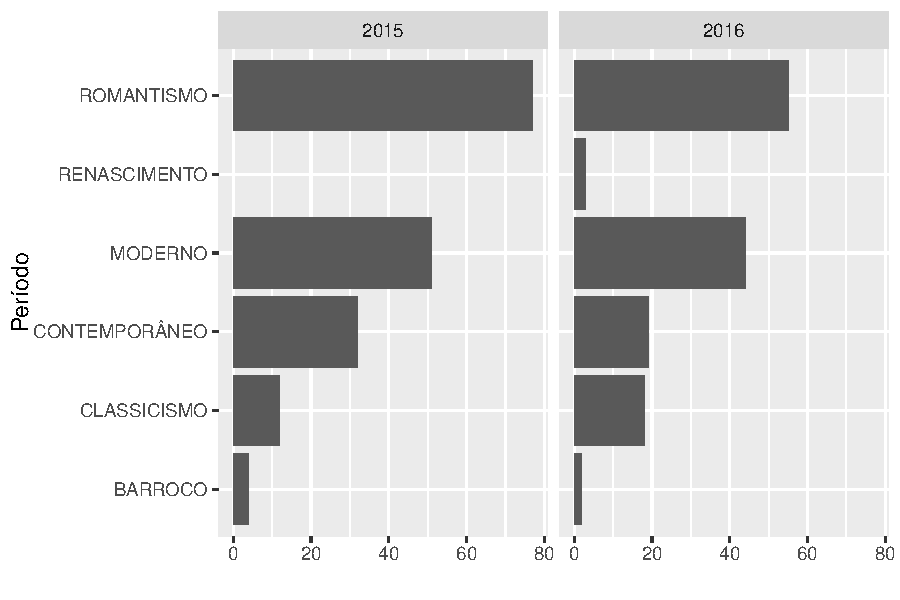
\includegraphics[scale=1]{periodo_peryear.pdf}
          \fonte{Elaborated by the author.}
        \end{figure}


        This proportion stays somewhat stable if we observe the main concert series (with the exception, of course, of the \textit{Fora de Série} thematic series). In Figure \ref{repertoire-perseries}, the Youth Concerts (in the middle column) seems to be the most balanced series. Allegro/Vivace and Presto/Veloce seem quite alike. In 2016, less Classical music has been made in these series. The genre was reserved in that year to \textit{Fora de Série} concerts. 

        \begin{figure}[!h]
          \centering
          \caption{Repertoire by series}
          \label{repertoire-perseries}
          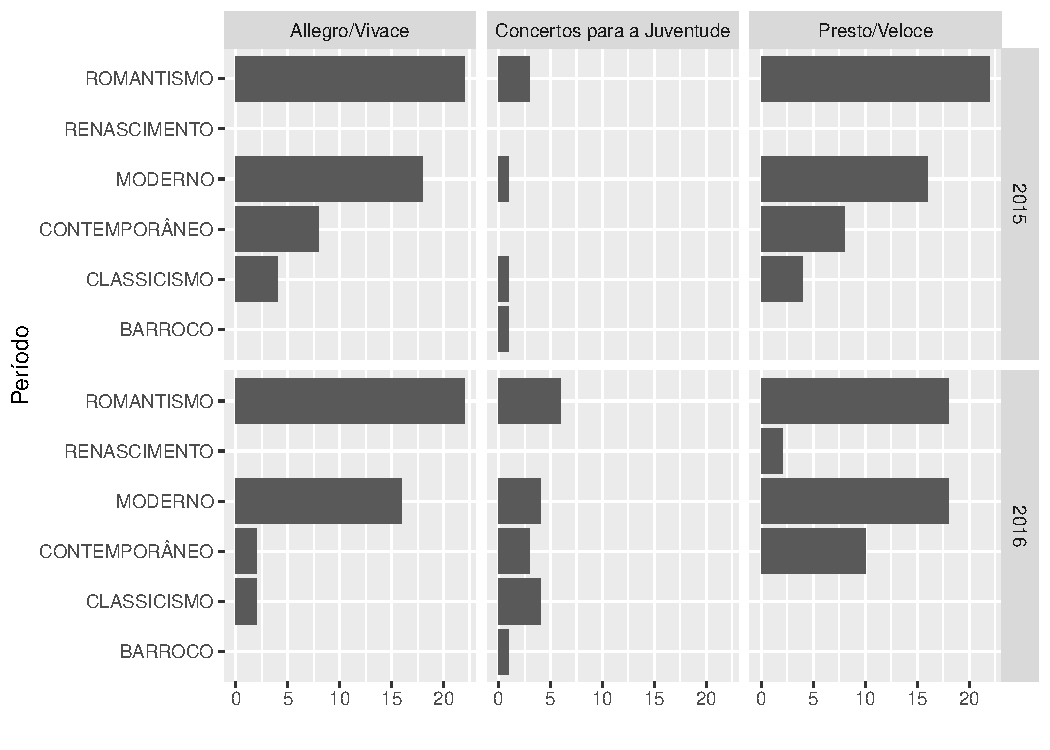
\includegraphics[scale=1]{periodo_perserie_year.pdf}
          \fonte{Elaborated by the author.}
        \end{figure}


        In order to investigate the consumption, the 2016 results report gives us the number of seats available and the number of tickets sold to calculate the occupancy rate. At first, we are tented to believe that the consumption of the concerts is mostly related by the chosen repertoire which, therefore, would reflect on the concert series. Nevertheless, because of the change in the concerts offering since 2015, we believe that the weekday has a larger impact on consumption. Linear models showed that the series has a bigger explanatory power on consumption (cf. Table \ref{concert-consumption-models}). The models were estimated with the occupancy rate as the dependent variable and only for 2016\footnote{Unfortunately, the number of seats available is only reported in 2016's reports. In order to make our further analysis more robust, we estimated the seats available for 2015 given that the venues, the weekdays of the concerts and the series were the same as 2016. A technical description of the estimation procedure is given in the appendix.}.

        \begin{table}[!ht]
          \ibgetab{
            \centering
            \caption{Concert consumption - Linear models}
            \label{concert-consumption-models}
          }
          {\begin{tabular}{l c c }
             \hline
             & Model 1 & Model 2 \\
             \hline
             (Intercept)                                        & $85.28^{***}$ & $93.36^{***}$  \\
             & $(1.84)$      & $(1.46)$       \\
             \textbf{Weekdays} & & \\
             Sunday & $14.72^{***}$ &                \\
             & $(3.98)$      &                \\
             Thursday  & $4.59$        &                \\
             & $(2.58)$      &                \\
             Saturday  & $12.15^{***}$ &                \\
             & $(3.10)$      &                \\
             \textbf{Concert series} & & \\
             Concertos para a Juventude                    &               & $6.64^{*}$     \\
             &               & $(3.21)$       \\
             Fora de Série                                 &               & $6.13^{*}$     \\
             &               & $(2.65)$       \\
             Presto/Veloce                                 &               & $-11.26^{***}$ \\
             &               & $(2.05)$       \\
             \hline
             R$^2$                                              & 0.28          & 0.53           \\
             Adj. R$^2$                                         & 0.25          & 0.50           \\
             Num. obs.                                          & 63            & 63             \\
             RMSE                                               & 8.64          & 7.01           \\
             \hline
             \multicolumn{3}{l}{\scriptsize{$^{***}p<0.001$, $^{**}p<0.01$, $^*p<0.05$}}
           \end{tabular}
         }
         {\fonte{Elaborated by the author.}}
       \end{table}


       % Talk about occupancy rate by series. Run the analysis in R.
       On Table \ref{occupancy-table} we can observe that weekend concerts have higher occupancy rate than on weekdays. ....................

       % latex table generated in R 3.4.3 by xtable 1.8-2 package
       % Mon Jan 15 14:19:21 2018
       \begin{table}[ht]
         \ibgetab{
           \centering
           \caption{Occupancy rate -- 2015-16}
           \label{occupancy-table}
         }
         {\begin{tabular}{lrrrrr}
            \hline
            \multicolumn{6}{l}{\textbf{By Concert Series}} \\
            \hline
            Concert Series & mean & median & sd & min & max \\ 
            \hline
            Allegro/Vivace & 91.45 & 92.11 & 6.13 & 70.56 & 99.20 \\ 
            Concertos para a Juventude & 99.52 & 100.00 & 0.57 & 98.19 & 100.00 \\
            Fora de Série & 99.19 & 99.67 & 1.12 & 96.05 & 100.00 \\
            Presto/Veloce & 79.62 & 80.25 & 11.87 & 56.15 & 98.03 \\
            \hline
            \multicolumn{6}{l}{\textbf{By Weekday}} \\
            \hline
            Weekday & mean & median & sd & min & max \\
            \hline
            Sunday & 99.52 & 100.00 & 0.57 & 98.19 & 100.00 \\ 
            Thursday & 89.86 & 91.01 & 7.49 & 66.55 & 99.20 \\ 
            Saturday & 98.40 & 99.20 & 2.43 & 90.29 & 100.00 \\ 
            Friday & 82.41 & 86.48 & 13.19 & 56.15 & 100.00 \\ 
            \hline
          \end{tabular}
        }
        {\fonte{Elaborated by the author.}}
      \end{table}
      










        \chapter{Next Steps}

        ..............









        
	
	
\postextual
\anexos

	
\citeoption{abnt-full-initials=yes}
\citeoption{abnt-and-type=&}
\bibliography{BIBDOUTORADO, abnt-options}

	\newpage
	\chapter*[Market Plane]{Appendix 1 -- The Market Plane}
	Here is a space for the beautiful intention of deriving the much very complicated White mathematical models\dots

        \newpage

        \chapter*[Questionnaire - individuals]{Appendix 2 -- Sociometric online questionnaire - individuals}

        [\textbf{First page}]
        
        Hello. Your are being invited to participate on the PhD research entitled ``The social construction of quality in a Brazilian Classical Music market'' by Neylson Crepalde. We can assure total confidentiality of participants. Because this is a network study, we will need to know the name of some of your colleagues/coworkers. However, NO NAMES WILL BE DISCLOSED in the research report or in scientific papers published with this data.

        This research has Prof. Dr. Silvio Salej Higgins as advisor and Prof. Dr. Emmanuel Lazega as co-advisor. Your participation is voluntary and you will not have any onus because of it.

        In case of any doubts, please, write to \url{neylsoncrepalde@gmail.com}.

        At any time, it is possible to withdraw your participation from the study. In case you decide not to participate after you have answered to this online questionnaire, your data will be excluded from our database. We urge, however, that your participation is extremely important to the success of this research. Thank you for collaborating!

        In case you agree on participating, click under CONTINUE to access the questions.

        [\textbf{Second page - General Information}] % UNDER CONSTRUCTION......

        \begin{enumerate}
        \item Full name: 
        \item E-mail address:

        \item What is your Gender?
          \begin{itemize}
          \item Male
          \item Female
          \item Other
          \end{itemize}

        \item What is your highest degree?
          \begin{itemize}
          \item High school - incomplete
          \item High school - complete
          \item Undergraduate - incomplete
          \item Undergraduate - complete
          \item Masters - incomplete
          \item Masters - complete
          \item PhD - incomplete
          \item PhD - complete
          \end{itemize}

        \item How do you consider yourself regarding skin colour?
          \begin{itemize}
          \item White
          \item Black
          \item Brow
          \item Asian
          \item Indigenous
          \item Other
          \end{itemize}

        \item How old are you?
          
        \item Where do you live? Please answer with City and neighborhood as in the example: Belo Horizonte, Savassi; Paris, 14th.
          
        \item What is your civil state?
          \begin{itemize}
          \item Married
          \item Single
          \item Divorced
          \item Widower
          \end{itemize}

         
        \item Do you have children? How many?

        \item How many people live in your house/apartment?
        \item How many rooms does your house/apartment have?
          
        \item The house/apartment is
          \begin{itemize}
          \item your own - fully payed
          \item your own - still paying
          \item rented
          \item borrowed or ceded
          \end{itemize}
          
        \item Would you consider yourself as (check as many as you consider correct):
          \begin{itemize}
          \item Musician
          \item Music Teacher/Professor
          \item Public
          \item Critic
          \item Orchestra Staff
          \item Administrative
          \item Other (describe)
          \end{itemize}


        [\textbf{Third page - Vertical relations}]  

        \item Do you play in any orchestra? Which one(s)?
        \item Do you play in any groups or events regularly besides your work with the orchestra?
        \item Do you teach in any music school or college/university? Which?
        \item If you do teach, how many regular students do you have?
        \item Do you write critics or music articles regularly to any newspaper or online portal or other media?
        \item How many critics or articles do you publish per month?
        \item Do you work in the administrative sector of an orchestra? Which?
        \item Do you work in any company that is not an orchestra or an education institution? What is your position in this company?
        \item What is your income per month from the orchestras you play with?
        \item What is your total income per month considering your work with the orchestra and all the other activities that you do?

        \item How frequently do you attend concerts?
          \begin{itemize}
          \item Once or twice a year
          \item Once or twice each three months
          \item Once or twice every month
          \item Once a week
          \item More than once a week
          \end{itemize}

          
        \item The questions that follow are only related to musicians. Are you a musician?
          \begin{itemize}
          \item No -- Thank you very much for your participation!
          \item Yes -- Continue to the next questions.
          \end{itemize}


          
        [\textbf{Fourth page - Horizontal relations between individuals}]
        
        \item If you needed advise on a piece's interpretation, regardless of its period or style, to whom would you ask for an advise? List as many people you want to. Please, cite in this way: Person1 - Main activity, Person2 - Main activity, Person3 - Main activity.
        
        \item Do you often meet other people in social occasions outside work? Who do you meet? List as many people you want to. Please, cite in this way: Person1 - Main activity, Person2 - Main activity, Person3 - Main activity.

        \item If you were invited to help an orchestra hiring a musician for an excellent job offer, who would you recommend?

        \item If you were responsible for organizing a recital for you to play, regardless of the instrumentation of the works you could choose, who would you like to invite to play with you?

        \item To you, what are the orchestras in Belo Horizonte that have the highest quality? Please cite from the greatest to the poorest.

        \item Why the best orchestra that you pointed is the best? List as many reasons you can think of.


        

        [\textbf{Fifth page - Context}]
        
        \item In what country where you born?
        \item In what city where you born?
        \item For how many years do you study music?
        \item For how many years have you been working as a professional musician?
        \item What is your instrument or main musical activity (if you are a conductor or a singer, for instance)?
        \item In what institution did you receive most part of your musical training?
        \item With which teacher/professor did you spend most part of your musical training? 


        \end{enumerate}

        Thank you very much for your participation!


        \newpage

        \chapter*[Questionnaire - organizations]{Appendix 3 -- Sociometric questionnaire - organizations}

        Good day. I want to thank you very much for your participation and assure that it is extremely important for the success of this PhD research.

        \vspace{1cm}
        \begin{enumerate}
        \item Let's start with your professional partnerships. Could you name all the professionals that you relate with regularly? By professionals I mean every company with whom you have relations, economic or other, for example, advisement, collaboration, resources exchange, etc.

        \item What is the main activity of each of these professionals?

        \item I would like to retake each of this professionals that you mentioned. What is the relation that you would say you have with each one of them?
          \begin{itemize}
          \item A relation between supplier and customer, only.
          \item A partnership
          \item A collaboration
          \item An advisement relation
          \item Other
          \end{itemize}

        \item What is the organization's structure? Is there an organizational chart that I could consult?
        \item What is the organization's budget?     
          
        \item You did mention the State as one of your partners (What about the State?) How many contracts do you have with the State? What is it's share in your budget?
        \item What would you say is your organization's style within the market?

          \vspace{0.8cm}
          [\textbf{If it is an orchestra:}]
        \item In what spaces does the orchestra usually play? How many seats available?
        \item What is the ticket price for each of the concert series? Is there variation on ticket price according to the place in the concert room? How many tickets are made available with each price?
        \item How much does the organization spend with musicians paycheck?
        \item Besides musicians and guests paycheck, what would you say are other artistic expenses of a performance?

        \end{enumerate}

        Thank you very much for participating!
        


        \newpage

        \chapter*[Interview guide]{Appendix 4 -- Teacher/professor/hub's interview guide}

        Good day. I want to thank you very much for your participation and assure that it is extremely important for the success of this PhD research. Let's begin talking about your \textbf{musical training}:

        \begin{enumerate}
        \item Where did you study?
        \item What are your degrees in music?
        \item Do you think the place where you had musical training was important for the training itself? How?

          \vspace{1cm}
        Now, let's talk about your \textbf{students}.
        \item How many students do you have today?
        \item Are they working as professional musicians or they are only studying yet?
        \item How do you manage, in your classes, teaching about technical elements and interpretative elements?
        \item What do you do to make a student understand what does it take to have a ``good '' performance? Is this a difficult process or does it come naturally?
        \item To you, what are the higher quality orchestras in Belo Horizonte? Why?

          \vspace{1cm}
          Now, let's talk about your \textbf{carrer}.
        \item Beyond teaching, do you usually play on recitals or concertos?
        \item When you are performing with another musicians, how interpretative decisions are made?
        \end{enumerate}

        Thank you very much for participating!




        \chapter*[Random Forests]{Appendix 5 -- The Estimation of 2015's occupancy rate}

        In their periodic reports, Minas Gerais Philharmonic gives three major variables needed to investigate classical music consumption: number of tickets sold, number of seats available and the occupancy rate. Unfortunately, the number of seats available is only reported in 2016's reports. Given that since 2015 the venues, the concert series and the weekdays that concerts take place have exactly the same pattern, we can estimate the number of seats available for that year. This procedure is necessary because the number of seats available can vary according to the repertoire (chorus, no chorus), size of the orchestra and other factors.

        To do the estimation, we used a Random Forests algorithm in an R programming environment.

        EXPLAIN THE RANDOM FORESTS in a clear way..................

        

\end{document}
